\documentclass{book}
\usepackage[a4paper,top=2.5cm,bottom=2.5cm,left=2.5cm,right=2.5cm]{geometry}
\usepackage{makeidx}
\usepackage{natbib}
\usepackage{graphicx}
\usepackage{multicol}
\usepackage{float}
\usepackage{listings}
\usepackage{color}
\usepackage{ifthen}
\usepackage[table]{xcolor}
\usepackage{textcomp}
\usepackage{alltt}
\usepackage{ifpdf}
\ifpdf
\usepackage[pdftex,
            pagebackref=true,
            colorlinks=true,
            linkcolor=blue,
            unicode
           ]{hyperref}
\else
\usepackage[ps2pdf,
            pagebackref=true,
            colorlinks=true,
            linkcolor=blue,
            unicode
           ]{hyperref}
\usepackage{pspicture}
\fi
\usepackage[utf8]{inputenc}
\usepackage{mathptmx}
\usepackage[scaled=.90]{helvet}
\usepackage{courier}
\usepackage{sectsty}
\usepackage{amssymb}
\usepackage[titles]{tocloft}
\usepackage{doxygen}
\lstset{language=C++,inputencoding=utf8,basicstyle=\footnotesize,breaklines=true,breakatwhitespace=true,tabsize=8,numbers=left }
\makeindex
\setcounter{tocdepth}{3}
\renewcommand{\footrulewidth}{0.4pt}
\renewcommand{\familydefault}{\sfdefault}
\hfuzz=15pt
\setlength{\emergencystretch}{15pt}
\hbadness=750
\tolerance=750
\begin{document}
\hypersetup{pageanchor=false,citecolor=blue}
\begin{titlepage}
\vspace*{7cm}
\begin{center}
{\Large Curious Froggy \\[1ex]\large 1.\-0 }\\
\vspace*{1cm}
{\large Generated by Doxygen 1.8.1.2}\\
\vspace*{0.5cm}
{\small Thu May 23 2013 01:25:10}\\
\end{center}
\end{titlepage}
\clearemptydoublepage
\pagenumbering{roman}
\tableofcontents
\clearemptydoublepage
\pagenumbering{arabic}
\hypersetup{pageanchor=true,citecolor=blue}
\chapter{Data Structure Index}
\section{Data Structures}
Here are the data structures with brief descriptions\-:\begin{DoxyCompactList}
\item\contentsline{section}{\hyperlink{struct_background}{Background} \\*X et y sont les coordonnées du fond. img contient le B\-I\-T\-M\-A\-P du fond }{\pageref{struct_background}}{}
\item\contentsline{section}{\hyperlink{struct_barre}{Barre} \\*Celle ci est la strucuture de la barre de vie. x est la position de la \hyperlink{struct_barre}{Barre} en largeur et y en hauteur. Nous avons une seule \hyperlink{struct_barre}{Barre} de vie dans le jeu. img est le B\-I\-T\-M\-A\-P de cette \hyperlink{struct_barre}{Barre} puisque nous avons dans le jeu 6 vies donc nous avons ici 7 frames. (un pour vie = 0) }{\pageref{struct_barre}}{}
\item\contentsline{section}{\hyperlink{structbouton}{bouton} \\*Ceci est la structure d'un bouton qui doit apparaitre dans le menu. Elle contient les coordonnées du bouton et ses différents états (3 images) }{\pageref{structbouton}}{}
\item\contentsline{section}{\hyperlink{struct_calque}{Calque} \\*Img contient le B\-I\-T\-M\-A\-P du \hyperlink{struct_calque}{Calque} qui est qui est l'image du fond dans lequel les obstacles sont coloriés par des couleurs spécifiques (les trous en blanc de coordonnées 16777215, le plancher en bleu ciel de coordonnées 65535, la zone d'arrivée en orange de coordonnées 16850088 dans tous les stages à l'exception du stage 3 où seulement les obstacles sont coloriés en blanc de coordonnées 16777215) x est inversement proportionelle à fond.\-x. Lorsque cette dernière augmente calque.\-x diminue et inversement }{\pageref{struct_calque}}{}
\item\contentsline{section}{\hyperlink{struct_chargement}{Chargement} \\*Cette structure contient la barre de chargement du jeu avec ses 4 états d'avancement }{\pageref{struct_chargement}}{}
\item\contentsline{section}{\hyperlink{struct_coins}{Coins} \\*X et y sont les coordonnées des différentes pièces organisées dans les tableau int x\mbox{[}\mbox{]} et int y\mbox{[}\mbox{]}. img contient le B\-I\-T\-M\-A\-P du fond }{\pageref{struct_coins}}{}
\item\contentsline{section}{\hyperlink{struct_froggy}{Froggy} \\*X la position de \hyperlink{struct_froggy}{Froggy} en largeur et y en hauteur. Nous avons un seul sprite \hyperlink{struct_froggy}{Froggy} dans le jeu. img est le B\-I\-T\-M\-A\-P de ce pigeon puisque il contient 7 frames donc nous avons 7 images }{\pageref{struct_froggy}}{}
\item\contentsline{section}{\hyperlink{struct_game}{Game} \\*Cette structure contient les positions x et y des messages Game\-Over et You\-Win. Chacune d'eux contient deux etats mis dans 2 images dans le tableau B\-I\-T\-M\-A\-P $\ast$img\mbox{[}\mbox{]} }{\pageref{struct_game}}{}
\item\contentsline{section}{\hyperlink{structicone__stage1}{icone\-\_\-stage1} \\*Ceci est la structure d'une icône du stage 1 qui doit apparaitre dans le menu. Elle contient les coordonnées de l'icône }{\pageref{structicone__stage1}}{}
\item\contentsline{section}{\hyperlink{structicone__stage2}{icone\-\_\-stage2} \\*Ceci est la structure d'une icône du stage 2 qui doit apparaitre dans le menu. Elle contient les coordonnées de l'icône et ses différents états (2 images) verouillé ou ouvert }{\pageref{structicone__stage2}}{}
\item\contentsline{section}{\hyperlink{structicone__stage3}{icone\-\_\-stage3} \\*Ceci est la structure d'une icône du stage 3 qui doit apparaitre dans le menu. Elle contient les coordonnées de l'icône et ses différents états (2 images) verouillé ou ouvert }{\pageref{structicone__stage3}}{}
\item\contentsline{section}{\hyperlink{structicone__stage4}{icone\-\_\-stage4} \\*Ceci est la structure d'une icône du stage 4 qui doit apparaitre dans le menu. Elle contient les coordonnées de l'icône et ses différents états (2 images) verouillé ou ouvert }{\pageref{structicone__stage4}}{}
\item\contentsline{section}{\hyperlink{struct_numero}{Numero} \\*Cette structure contient des images de chiffres utilisées pour afficher le score. Puisque les chiffres vont de 0 à 9 donc nous avons ici 10 images }{\pageref{struct_numero}}{}
\item\contentsline{section}{\hyperlink{struct_pause}{Pause} \\*Cette structure est celle du menu de pause. Elle contient les coordonnées x et y du menu mais aussi les différents états (3 frames) }{\pageref{struct_pause}}{}
\item\contentsline{section}{\hyperlink{struct_pigeon}{Pigeon} \\*X la position du \hyperlink{struct_pigeon}{Pigeon} en largeur et y en hauteur. Nous avons un \hyperlink{struct_pigeon}{Pigeon} dans le jeu. img est le B\-I\-T\-M\-A\-P de ce \hyperlink{struct_pigeon}{Pigeon} puisque il contient 5 frames donc nous avons 5 images }{\pageref{struct_pigeon}}{}
\item\contentsline{section}{\hyperlink{struct_rat}{Rat} \\*X la position du rat en largeur et y en hauteur. Nous avons 4 voitures dans le jeu donc nous avons besoin de 4 x et de 4 y différents. img est le B\-I\-T\-M\-A\-P de cette voiture puisque elle contient 3 frames donc nous avons 3 images }{\pageref{struct_rat}}{}
\item\contentsline{section}{\hyperlink{struct_reine}{Reine} \\*X la position de reine en largeur et y en hauteur. Nous avons 3 reines dans le jeu donc nous avons besoin de 3 x et de 3 y différents. img est le B\-I\-T\-M\-A\-P de cette voiture puisque elle contient 5 positions donc nous avons 5 images }{\pageref{struct_reine}}{}
\item\contentsline{section}{\hyperlink{struct_serpent}{Serpent} \\*X la position du serpent en largeur et y en hauteur. Nous avons 3 serpents dans le jeu donc nous avons besoin de 3 x et de 3 y différents. img est le B\-I\-T\-M\-A\-P de ce serpent puisque il contient 5 positions donc nous avons 5 images }{\pageref{struct_serpent}}{}
\item\contentsline{section}{\hyperlink{struct_tete}{Tete} \\*Celle-\/ci est la structure de la tête de \hyperlink{struct_froggy}{Froggy} qui s'affiche en haut et à gauche de l'écran dans les stages 1,2 et 4 }{\pageref{struct_tete}}{}
\item\contentsline{section}{\hyperlink{struct_voiture}{Voiture} \\*X la position de la voiture en largeur et y en hauteur. Nous avons 4 voitures dans le jeu donc nous avons besoin de 4 x et de 4 y différents. img est le B\-I\-T\-M\-A\-P de cette voiture puisque elle contient 5 positions donc nous avons 5 images }{\pageref{struct_voiture}}{}
\end{DoxyCompactList}

\chapter{File Index}
\section{File List}
Here is a list of all documented files with brief descriptions\-:\begin{DoxyCompactList}
\item\contentsline{section}{\hyperlink{commun_8c}{commun.\-c} }{\pageref{commun_8c}}{}
\item\contentsline{section}{\hyperlink{commun_8h}{commun.\-h} }{\pageref{commun_8h}}{}
\item\contentsline{section}{\hyperlink{main_8c}{main.\-c} }{\pageref{main_8c}}{}
\item\contentsline{section}{\hyperlink{menu_8c}{menu.\-c} }{\pageref{menu_8c}}{}
\item\contentsline{section}{\hyperlink{menu_8h}{menu.\-h} }{\pageref{menu_8h}}{}
\item\contentsline{section}{\hyperlink{stage1_8c}{stage1.\-c} }{\pageref{stage1_8c}}{}
\item\contentsline{section}{\hyperlink{stage1_8h}{stage1.\-h} }{\pageref{stage1_8h}}{}
\item\contentsline{section}{\hyperlink{stage1__2_8c}{stage1\-\_\-2.\-c} }{\pageref{stage1__2_8c}}{}
\item\contentsline{section}{\hyperlink{stage1__2_8h}{stage1\-\_\-2.\-h} }{\pageref{stage1__2_8h}}{}
\item\contentsline{section}{\hyperlink{stage2_8c}{stage2.\-c} }{\pageref{stage2_8c}}{}
\item\contentsline{section}{\hyperlink{stage2_8h}{stage2.\-h} }{\pageref{stage2_8h}}{}
\item\contentsline{section}{\hyperlink{stage4_8c}{stage4.\-c} }{\pageref{stage4_8c}}{}
\item\contentsline{section}{\hyperlink{stage4_8h}{stage4.\-h} }{\pageref{stage4_8h}}{}
\end{DoxyCompactList}

\chapter{Data Structure Documentation}
\hypertarget{struct_background}{\section{Background Struct Reference}
\label{struct_background}\index{Background@{Background}}
}


x et y sont les coordonnées du fond. img contient le B\-I\-T\-M\-A\-P du fond  




{\ttfamily \#include $<$commun.\-h$>$}

\subsection*{Data Fields}
\begin{DoxyCompactItemize}
\item 
\hypertarget{struct_background_a6150e0515f7202e2fb518f7206ed97dc}{int {\bfseries x}}\label{struct_background_a6150e0515f7202e2fb518f7206ed97dc}

\item 
\hypertarget{struct_background_a0a2f84ed7838f07779ae24c5a9086d33}{int {\bfseries y}}\label{struct_background_a0a2f84ed7838f07779ae24c5a9086d33}

\item 
\hypertarget{struct_background_a8eae42c4d58d3ee6b9aa56d0071971fa}{B\-I\-T\-M\-A\-P $\ast$ {\bfseries img}}\label{struct_background_a8eae42c4d58d3ee6b9aa56d0071971fa}

\end{DoxyCompactItemize}


\subsection{Detailed Description}
x et y sont les coordonnées du fond. img contient le B\-I\-T\-M\-A\-P du fond 


\begin{DoxyItemize}
\item 
\end{DoxyItemize}

The documentation for this struct was generated from the following file\-:\begin{DoxyCompactItemize}
\item 
\hyperlink{commun_8h}{commun.\-h}\end{DoxyCompactItemize}

\hypertarget{struct_barre}{\section{Barre Struct Reference}
\label{struct_barre}\index{Barre@{Barre}}
}


Celle ci est la strucuture de la barre de vie. x est la position de la \hyperlink{struct_barre}{Barre} en largeur et y en hauteur. Nous avons une seule \hyperlink{struct_barre}{Barre} de vie dans le jeu. img est le B\-I\-T\-M\-A\-P de cette \hyperlink{struct_barre}{Barre} puisque nous avons dans le jeu 6 vies donc nous avons ici 7 frames. (un pour vie = 0)  




{\ttfamily \#include $<$commun.\-h$>$}

\subsection*{Data Fields}
\begin{DoxyCompactItemize}
\item 
\hypertarget{struct_barre_a6150e0515f7202e2fb518f7206ed97dc}{int {\bfseries x}}\label{struct_barre_a6150e0515f7202e2fb518f7206ed97dc}

\item 
\hypertarget{struct_barre_a0a2f84ed7838f07779ae24c5a9086d33}{int {\bfseries y}}\label{struct_barre_a0a2f84ed7838f07779ae24c5a9086d33}

\item 
\hypertarget{struct_barre_ab6b4c00f9aaa715f23d59ed627e5a92d}{B\-I\-T\-M\-A\-P $\ast$ {\bfseries img} \mbox{[}7\mbox{]}}\label{struct_barre_ab6b4c00f9aaa715f23d59ed627e5a92d}

\end{DoxyCompactItemize}


\subsection{Detailed Description}
Celle ci est la strucuture de la barre de vie. x est la position de la \hyperlink{struct_barre}{Barre} en largeur et y en hauteur. Nous avons une seule \hyperlink{struct_barre}{Barre} de vie dans le jeu. img est le B\-I\-T\-M\-A\-P de cette \hyperlink{struct_barre}{Barre} puisque nous avons dans le jeu 6 vies donc nous avons ici 7 frames. (un pour vie = 0) 


\begin{DoxyItemize}
\item 
\end{DoxyItemize}

The documentation for this struct was generated from the following file\-:\begin{DoxyCompactItemize}
\item 
\hyperlink{commun_8h}{commun.\-h}\end{DoxyCompactItemize}

\hypertarget{structbouton}{\section{bouton Struct Reference}
\label{structbouton}\index{bouton@{bouton}}
}


Ceci est la structure d'un bouton qui doit apparaitre dans le menu. Elle contient les coordonnées du bouton et ses différents états (3 images)  




{\ttfamily \#include $<$menu.\-h$>$}

\subsection*{Data Fields}
\begin{DoxyCompactItemize}
\item 
\hypertarget{structbouton_a6150e0515f7202e2fb518f7206ed97dc}{int {\bfseries x}}\label{structbouton_a6150e0515f7202e2fb518f7206ed97dc}

\item 
\hypertarget{structbouton_a0a2f84ed7838f07779ae24c5a9086d33}{int {\bfseries y}}\label{structbouton_a0a2f84ed7838f07779ae24c5a9086d33}

\item 
\hypertarget{structbouton_a99933deee119efe612d38cf6759af35e}{B\-I\-T\-M\-A\-P $\ast$ {\bfseries img} \mbox{[}3\mbox{]}}\label{structbouton_a99933deee119efe612d38cf6759af35e}

\end{DoxyCompactItemize}


\subsection{Detailed Description}
Ceci est la structure d'un bouton qui doit apparaitre dans le menu. Elle contient les coordonnées du bouton et ses différents états (3 images) 


\begin{DoxyItemize}
\item 
\end{DoxyItemize}

The documentation for this struct was generated from the following file\-:\begin{DoxyCompactItemize}
\item 
\hyperlink{menu_8h}{menu.\-h}\end{DoxyCompactItemize}

\hypertarget{struct_calque}{\section{Calque Struct Reference}
\label{struct_calque}\index{Calque@{Calque}}
}


img contient le B\-I\-T\-M\-A\-P du \hyperlink{struct_calque}{Calque} qui est qui est l'image du fond dans lequel les obstacles sont coloriés par des couleurs spécifiques (les trous en blanc de coordonnées 16777215, le plancher en bleu ciel de coordonnées 65535, la zone d'arrivée en orange de coordonnées 16850088 dans tous les stages à l'exception du stage 3 où seulement les obstacles sont coloriés en blanc de coordonnées 16777215) x est inversement proportionelle à fond.\-x. Lorsque cette dernière augmente calque.\-x diminue et inversement  




{\ttfamily \#include $<$commun.\-h$>$}

\subsection*{Data Fields}
\begin{DoxyCompactItemize}
\item 
\hypertarget{struct_calque_a8eae42c4d58d3ee6b9aa56d0071971fa}{B\-I\-T\-M\-A\-P $\ast$ {\bfseries img}}\label{struct_calque_a8eae42c4d58d3ee6b9aa56d0071971fa}

\item 
\hypertarget{struct_calque_a6150e0515f7202e2fb518f7206ed97dc}{int {\bfseries x}}\label{struct_calque_a6150e0515f7202e2fb518f7206ed97dc}

\item 
\hypertarget{struct_calque_a0a2f84ed7838f07779ae24c5a9086d33}{int {\bfseries y}}\label{struct_calque_a0a2f84ed7838f07779ae24c5a9086d33}

\end{DoxyCompactItemize}


\subsection{Detailed Description}
img contient le B\-I\-T\-M\-A\-P du \hyperlink{struct_calque}{Calque} qui est qui est l'image du fond dans lequel les obstacles sont coloriés par des couleurs spécifiques (les trous en blanc de coordonnées 16777215, le plancher en bleu ciel de coordonnées 65535, la zone d'arrivée en orange de coordonnées 16850088 dans tous les stages à l'exception du stage 3 où seulement les obstacles sont coloriés en blanc de coordonnées 16777215) x est inversement proportionelle à fond.\-x. Lorsque cette dernière augmente calque.\-x diminue et inversement 


\begin{DoxyItemize}
\item 
\end{DoxyItemize}

The documentation for this struct was generated from the following file\-:\begin{DoxyCompactItemize}
\item 
\hyperlink{commun_8h}{commun.\-h}\end{DoxyCompactItemize}

\hypertarget{struct_chargement}{\section{Chargement Struct Reference}
\label{struct_chargement}\index{Chargement@{Chargement}}
}


Cette structure contient la barre de chargement du jeu avec ses 4 états d'avancement.  




{\ttfamily \#include $<$commun.\-h$>$}

\subsection*{Data Fields}
\begin{DoxyCompactItemize}
\item 
\hypertarget{struct_chargement_acc64649e1a4857389f509f6d06b93732}{B\-I\-T\-M\-A\-P $\ast$ {\bfseries img} \mbox{[}4\mbox{]}}\label{struct_chargement_acc64649e1a4857389f509f6d06b93732}

\item 
\hypertarget{struct_chargement_a6150e0515f7202e2fb518f7206ed97dc}{int {\bfseries x}}\label{struct_chargement_a6150e0515f7202e2fb518f7206ed97dc}

\item 
\hypertarget{struct_chargement_a0a2f84ed7838f07779ae24c5a9086d33}{int {\bfseries y}}\label{struct_chargement_a0a2f84ed7838f07779ae24c5a9086d33}

\end{DoxyCompactItemize}


\subsection{Detailed Description}
Cette structure contient la barre de chargement du jeu avec ses 4 états d'avancement. 


\begin{DoxyItemize}
\item 
\end{DoxyItemize}

The documentation for this struct was generated from the following file\-:\begin{DoxyCompactItemize}
\item 
\hyperlink{commun_8h}{commun.\-h}\end{DoxyCompactItemize}

\hypertarget{struct_coins}{\section{Coins Struct Reference}
\label{struct_coins}\index{Coins@{Coins}}
}


x et y sont les coordonnées des différentes pièces organisées dans les tableau int x\mbox{[}\mbox{]} et int y\mbox{[}\mbox{]}. img contient le B\-I\-T\-M\-A\-P du fond  




{\ttfamily \#include $<$commun.\-h$>$}

\subsection*{Data Fields}
\begin{DoxyCompactItemize}
\item 
\hypertarget{struct_coins_a5d9353e006bc18a21e8cbdee87d36a2f}{int {\bfseries x} \mbox{[}100\mbox{]}}\label{struct_coins_a5d9353e006bc18a21e8cbdee87d36a2f}

\item 
\hypertarget{struct_coins_a76e44bc53d2efde76380be19dc9ebbc3}{int {\bfseries y} \mbox{[}100\mbox{]}}\label{struct_coins_a76e44bc53d2efde76380be19dc9ebbc3}

\item 
\hypertarget{struct_coins_a8eae42c4d58d3ee6b9aa56d0071971fa}{B\-I\-T\-M\-A\-P $\ast$ {\bfseries img}}\label{struct_coins_a8eae42c4d58d3ee6b9aa56d0071971fa}

\end{DoxyCompactItemize}


\subsection{Detailed Description}
x et y sont les coordonnées des différentes pièces organisées dans les tableau int x\mbox{[}\mbox{]} et int y\mbox{[}\mbox{]}. img contient le B\-I\-T\-M\-A\-P du fond 


\begin{DoxyItemize}
\item 
\end{DoxyItemize}

The documentation for this struct was generated from the following file\-:\begin{DoxyCompactItemize}
\item 
\hyperlink{commun_8h}{commun.\-h}\end{DoxyCompactItemize}

\hypertarget{struct_froggy}{\section{Froggy Struct Reference}
\label{struct_froggy}\index{Froggy@{Froggy}}
}


x la position de \hyperlink{struct_froggy}{Froggy} en largeur et y en hauteur. Nous avons un seul sprite \hyperlink{struct_froggy}{Froggy} dans le jeu. img est le B\-I\-T\-M\-A\-P de ce pigeon puisque il contient 7 frames donc nous avons 7 images.  




{\ttfamily \#include $<$commun.\-h$>$}

\subsection*{Data Fields}
\begin{DoxyCompactItemize}
\item 
\hypertarget{struct_froggy_a6150e0515f7202e2fb518f7206ed97dc}{int {\bfseries x}}\label{struct_froggy_a6150e0515f7202e2fb518f7206ed97dc}

\item 
\hypertarget{struct_froggy_a0a2f84ed7838f07779ae24c5a9086d33}{int {\bfseries y}}\label{struct_froggy_a0a2f84ed7838f07779ae24c5a9086d33}

\item 
\hypertarget{struct_froggy_ab6b4c00f9aaa715f23d59ed627e5a92d}{B\-I\-T\-M\-A\-P $\ast$ {\bfseries img} \mbox{[}7\mbox{]}}\label{struct_froggy_ab6b4c00f9aaa715f23d59ed627e5a92d}

\end{DoxyCompactItemize}


\subsection{Detailed Description}
x la position de \hyperlink{struct_froggy}{Froggy} en largeur et y en hauteur. Nous avons un seul sprite \hyperlink{struct_froggy}{Froggy} dans le jeu. img est le B\-I\-T\-M\-A\-P de ce pigeon puisque il contient 7 frames donc nous avons 7 images. 


\begin{DoxyItemize}
\item 
\end{DoxyItemize}

The documentation for this struct was generated from the following file\-:\begin{DoxyCompactItemize}
\item 
\hyperlink{commun_8h}{commun.\-h}\end{DoxyCompactItemize}

\hypertarget{struct_game}{\section{Game Struct Reference}
\label{struct_game}\index{Game@{Game}}
}


Cette structure contient les positions x et y des messages Game\-Over et You\-Win. Chacune d'eux contient deux etats mis dans 2 images dans le tableau B\-I\-T\-M\-A\-P $\ast$img\mbox{[}\mbox{]}.  




{\ttfamily \#include $<$commun.\-h$>$}

\subsection*{Data Fields}
\begin{DoxyCompactItemize}
\item 
\hypertarget{struct_game_a6150e0515f7202e2fb518f7206ed97dc}{int {\bfseries x}}\label{struct_game_a6150e0515f7202e2fb518f7206ed97dc}

\item 
\hypertarget{struct_game_a0a2f84ed7838f07779ae24c5a9086d33}{int {\bfseries y}}\label{struct_game_a0a2f84ed7838f07779ae24c5a9086d33}

\item 
\hypertarget{struct_game_ab1bd34bcded6c8709b926189b4f50c2c}{B\-I\-T\-M\-A\-P $\ast$ {\bfseries img} \mbox{[}2\mbox{]}}\label{struct_game_ab1bd34bcded6c8709b926189b4f50c2c}

\end{DoxyCompactItemize}


\subsection{Detailed Description}
Cette structure contient les positions x et y des messages Game\-Over et You\-Win. Chacune d'eux contient deux etats mis dans 2 images dans le tableau B\-I\-T\-M\-A\-P $\ast$img\mbox{[}\mbox{]}. 


\begin{DoxyItemize}
\item 
\end{DoxyItemize}

The documentation for this struct was generated from the following file\-:\begin{DoxyCompactItemize}
\item 
\hyperlink{commun_8h}{commun.\-h}\end{DoxyCompactItemize}

\hypertarget{structicone__stage1}{\section{icone\-\_\-stage1 Struct Reference}
\label{structicone__stage1}\index{icone\-\_\-stage1@{icone\-\_\-stage1}}
}


Ceci est la structure d'une icône du stage 1 qui doit apparaitre dans le menu. Elle contient les coordonnées de l'icône.  




{\ttfamily \#include $<$menu.\-h$>$}

\subsection*{Data Fields}
\begin{DoxyCompactItemize}
\item 
\hypertarget{structicone__stage1_a6150e0515f7202e2fb518f7206ed97dc}{int {\bfseries x}}\label{structicone__stage1_a6150e0515f7202e2fb518f7206ed97dc}

\item 
\hypertarget{structicone__stage1_a0a2f84ed7838f07779ae24c5a9086d33}{int {\bfseries y}}\label{structicone__stage1_a0a2f84ed7838f07779ae24c5a9086d33}

\item 
\hypertarget{structicone__stage1_a8eae42c4d58d3ee6b9aa56d0071971fa}{B\-I\-T\-M\-A\-P $\ast$ {\bfseries img}}\label{structicone__stage1_a8eae42c4d58d3ee6b9aa56d0071971fa}

\end{DoxyCompactItemize}


\subsection{Detailed Description}
Ceci est la structure d'une icône du stage 1 qui doit apparaitre dans le menu. Elle contient les coordonnées de l'icône. 


\begin{DoxyItemize}
\item 
\end{DoxyItemize}

The documentation for this struct was generated from the following file\-:\begin{DoxyCompactItemize}
\item 
\hyperlink{menu_8h}{menu.\-h}\end{DoxyCompactItemize}

\hypertarget{structicone__stage2}{\section{icone\-\_\-stage2 Struct Reference}
\label{structicone__stage2}\index{icone\-\_\-stage2@{icone\-\_\-stage2}}
}


Ceci est la structure d'une icône du stage 2 qui doit apparaitre dans le menu. Elle contient les coordonnées de l'icône et ses différents états (2 images) verouillé ou ouvert.  




{\ttfamily \#include $<$menu.\-h$>$}

\subsection*{Data Fields}
\begin{DoxyCompactItemize}
\item 
\hypertarget{structicone__stage2_a6150e0515f7202e2fb518f7206ed97dc}{int {\bfseries x}}\label{structicone__stage2_a6150e0515f7202e2fb518f7206ed97dc}

\item 
\hypertarget{structicone__stage2_a0a2f84ed7838f07779ae24c5a9086d33}{int {\bfseries y}}\label{structicone__stage2_a0a2f84ed7838f07779ae24c5a9086d33}

\item 
\hypertarget{structicone__stage2_ab1bd34bcded6c8709b926189b4f50c2c}{B\-I\-T\-M\-A\-P $\ast$ {\bfseries img} \mbox{[}2\mbox{]}}\label{structicone__stage2_ab1bd34bcded6c8709b926189b4f50c2c}

\end{DoxyCompactItemize}


\subsection{Detailed Description}
Ceci est la structure d'une icône du stage 2 qui doit apparaitre dans le menu. Elle contient les coordonnées de l'icône et ses différents états (2 images) verouillé ou ouvert. 


\begin{DoxyItemize}
\item 
\end{DoxyItemize}

The documentation for this struct was generated from the following file\-:\begin{DoxyCompactItemize}
\item 
\hyperlink{menu_8h}{menu.\-h}\end{DoxyCompactItemize}

\hypertarget{structicone__stage3}{\section{icone\-\_\-stage3 Struct Reference}
\label{structicone__stage3}\index{icone\-\_\-stage3@{icone\-\_\-stage3}}
}


Ceci est la structure d'une icône du stage 3 qui doit apparaitre dans le menu. Elle contient les coordonnées de l'icône et ses différents états (2 images) verouillé ou ouvert.  




{\ttfamily \#include $<$menu.\-h$>$}

\subsection*{Data Fields}
\begin{DoxyCompactItemize}
\item 
\hypertarget{structicone__stage3_a6150e0515f7202e2fb518f7206ed97dc}{int {\bfseries x}}\label{structicone__stage3_a6150e0515f7202e2fb518f7206ed97dc}

\item 
\hypertarget{structicone__stage3_a0a2f84ed7838f07779ae24c5a9086d33}{int {\bfseries y}}\label{structicone__stage3_a0a2f84ed7838f07779ae24c5a9086d33}

\item 
\hypertarget{structicone__stage3_ab1bd34bcded6c8709b926189b4f50c2c}{B\-I\-T\-M\-A\-P $\ast$ {\bfseries img} \mbox{[}2\mbox{]}}\label{structicone__stage3_ab1bd34bcded6c8709b926189b4f50c2c}

\end{DoxyCompactItemize}


\subsection{Detailed Description}
Ceci est la structure d'une icône du stage 3 qui doit apparaitre dans le menu. Elle contient les coordonnées de l'icône et ses différents états (2 images) verouillé ou ouvert. 


\begin{DoxyItemize}
\item 
\end{DoxyItemize}

The documentation for this struct was generated from the following file\-:\begin{DoxyCompactItemize}
\item 
\hyperlink{menu_8h}{menu.\-h}\end{DoxyCompactItemize}

\hypertarget{structicone__stage4}{\section{icone\-\_\-stage4 Struct Reference}
\label{structicone__stage4}\index{icone\-\_\-stage4@{icone\-\_\-stage4}}
}


Ceci est la structure d'une icône du stage 4 qui doit apparaitre dans le menu. Elle contient les coordonnées de l'icône et ses différents états (2 images) verouillé ou ouvert.  




{\ttfamily \#include $<$menu.\-h$>$}

\subsection*{Data Fields}
\begin{DoxyCompactItemize}
\item 
\hypertarget{structicone__stage4_a6150e0515f7202e2fb518f7206ed97dc}{int {\bfseries x}}\label{structicone__stage4_a6150e0515f7202e2fb518f7206ed97dc}

\item 
\hypertarget{structicone__stage4_a0a2f84ed7838f07779ae24c5a9086d33}{int {\bfseries y}}\label{structicone__stage4_a0a2f84ed7838f07779ae24c5a9086d33}

\item 
\hypertarget{structicone__stage4_ab1bd34bcded6c8709b926189b4f50c2c}{B\-I\-T\-M\-A\-P $\ast$ {\bfseries img} \mbox{[}2\mbox{]}}\label{structicone__stage4_ab1bd34bcded6c8709b926189b4f50c2c}

\end{DoxyCompactItemize}


\subsection{Detailed Description}
Ceci est la structure d'une icône du stage 4 qui doit apparaitre dans le menu. Elle contient les coordonnées de l'icône et ses différents états (2 images) verouillé ou ouvert. 


\begin{DoxyItemize}
\item 
\end{DoxyItemize}

The documentation for this struct was generated from the following file\-:\begin{DoxyCompactItemize}
\item 
\hyperlink{menu_8h}{menu.\-h}\end{DoxyCompactItemize}

\hypertarget{struct_numero}{\section{Numero Struct Reference}
\label{struct_numero}\index{Numero@{Numero}}
}


Cette structure contient des images de chiffres utilisées pour afficher le score. Puisque les chiffres vont de 0 à 9 donc nous avons ici 10 images.  




{\ttfamily \#include $<$commun.\-h$>$}

\subsection*{Data Fields}
\begin{DoxyCompactItemize}
\item 
\hypertarget{struct_numero_aab65b1554dcc65b6fd50474af61ac3fb}{B\-I\-T\-M\-A\-P $\ast$ {\bfseries img} \mbox{[}10\mbox{]}}\label{struct_numero_aab65b1554dcc65b6fd50474af61ac3fb}

\end{DoxyCompactItemize}


\subsection{Detailed Description}
Cette structure contient des images de chiffres utilisées pour afficher le score. Puisque les chiffres vont de 0 à 9 donc nous avons ici 10 images. 


\begin{DoxyItemize}
\item 
\end{DoxyItemize}

The documentation for this struct was generated from the following file\-:\begin{DoxyCompactItemize}
\item 
\hyperlink{commun_8h}{commun.\-h}\end{DoxyCompactItemize}

\hypertarget{struct_pause}{\section{Pause Struct Reference}
\label{struct_pause}\index{Pause@{Pause}}
}


Cette structure est celle du menu de pause. Elle contient les coordonnées x et y du menu mais aussi les différents états (3 frames)  




{\ttfamily \#include $<$commun.\-h$>$}

\subsection*{Data Fields}
\begin{DoxyCompactItemize}
\item 
\hypertarget{struct_pause_a6150e0515f7202e2fb518f7206ed97dc}{int {\bfseries x}}\label{struct_pause_a6150e0515f7202e2fb518f7206ed97dc}

\item 
\hypertarget{struct_pause_a0a2f84ed7838f07779ae24c5a9086d33}{int {\bfseries y}}\label{struct_pause_a0a2f84ed7838f07779ae24c5a9086d33}

\item 
\hypertarget{struct_pause_a99933deee119efe612d38cf6759af35e}{B\-I\-T\-M\-A\-P $\ast$ {\bfseries img} \mbox{[}3\mbox{]}}\label{struct_pause_a99933deee119efe612d38cf6759af35e}

\end{DoxyCompactItemize}


\subsection{Detailed Description}
Cette structure est celle du menu de pause. Elle contient les coordonnées x et y du menu mais aussi les différents états (3 frames) 


\begin{DoxyItemize}
\item 
\end{DoxyItemize}

The documentation for this struct was generated from the following file\-:\begin{DoxyCompactItemize}
\item 
\hyperlink{commun_8h}{commun.\-h}\end{DoxyCompactItemize}

\hypertarget{struct_pigeon}{\section{Pigeon Struct Reference}
\label{struct_pigeon}\index{Pigeon@{Pigeon}}
}


x la position du \hyperlink{struct_pigeon}{Pigeon} en largeur et y en hauteur. Nous avons un \hyperlink{struct_pigeon}{Pigeon} dans le jeu. img est le B\-I\-T\-M\-A\-P de ce \hyperlink{struct_pigeon}{Pigeon} puisque il contient 5 frames donc nous avons 5 images.  




{\ttfamily \#include $<$stage2.\-h$>$}

\subsection*{Data Fields}
\begin{DoxyCompactItemize}
\item 
\hypertarget{struct_pigeon_a4206cc246eae0a153dd37253a8835ac9}{B\-I\-T\-M\-A\-P $\ast$ {\bfseries img} \mbox{[}5\mbox{]}}\label{struct_pigeon_a4206cc246eae0a153dd37253a8835ac9}

\item 
\hypertarget{struct_pigeon_a6150e0515f7202e2fb518f7206ed97dc}{int {\bfseries x}}\label{struct_pigeon_a6150e0515f7202e2fb518f7206ed97dc}

\item 
\hypertarget{struct_pigeon_a0a2f84ed7838f07779ae24c5a9086d33}{int {\bfseries y}}\label{struct_pigeon_a0a2f84ed7838f07779ae24c5a9086d33}

\end{DoxyCompactItemize}


\subsection{Detailed Description}
x la position du \hyperlink{struct_pigeon}{Pigeon} en largeur et y en hauteur. Nous avons un \hyperlink{struct_pigeon}{Pigeon} dans le jeu. img est le B\-I\-T\-M\-A\-P de ce \hyperlink{struct_pigeon}{Pigeon} puisque il contient 5 frames donc nous avons 5 images. 


\begin{DoxyItemize}
\item 
\end{DoxyItemize}

The documentation for this struct was generated from the following file\-:\begin{DoxyCompactItemize}
\item 
\hyperlink{stage2_8h}{stage2.\-h}\end{DoxyCompactItemize}

\hypertarget{struct_rat}{\section{Rat Struct Reference}
\label{struct_rat}\index{Rat@{Rat}}
}


x la position du rat en largeur et y en hauteur. Nous avons 4 voitures dans le jeu donc nous avons besoin de 4 x et de 4 y différents. img est le B\-I\-T\-M\-A\-P de cette voiture puisque elle contient 3 frames donc nous avons 3 images.  




{\ttfamily \#include $<$stage1.\-h$>$}

\subsection*{Data Fields}
\begin{DoxyCompactItemize}
\item 
\hypertarget{struct_rat_a99933deee119efe612d38cf6759af35e}{B\-I\-T\-M\-A\-P $\ast$ {\bfseries img} \mbox{[}3\mbox{]}}\label{struct_rat_a99933deee119efe612d38cf6759af35e}

\item 
\hypertarget{struct_rat_ab497c9cc64d8241f54bee95e694ff756}{int {\bfseries x} \mbox{[}4\mbox{]}}\label{struct_rat_ab497c9cc64d8241f54bee95e694ff756}

\item 
\hypertarget{struct_rat_afbc004b650e7331b8b87243a689dc765}{int {\bfseries y} \mbox{[}4\mbox{]}}\label{struct_rat_afbc004b650e7331b8b87243a689dc765}

\end{DoxyCompactItemize}


\subsection{Detailed Description}
x la position du rat en largeur et y en hauteur. Nous avons 4 voitures dans le jeu donc nous avons besoin de 4 x et de 4 y différents. img est le B\-I\-T\-M\-A\-P de cette voiture puisque elle contient 3 frames donc nous avons 3 images. 


\begin{DoxyItemize}
\item 
\end{DoxyItemize}

The documentation for this struct was generated from the following file\-:\begin{DoxyCompactItemize}
\item 
\hyperlink{stage1_8h}{stage1.\-h}\end{DoxyCompactItemize}

\hypertarget{struct_reine}{\section{Reine Struct Reference}
\label{struct_reine}\index{Reine@{Reine}}
}


x la position de reine en largeur et y en hauteur. Nous avons 3 reines dans le jeu donc nous avons besoin de 3 x et de 3 y différents. img est le B\-I\-T\-M\-A\-P de cette voiture puisque elle contient 5 positions donc nous avons 5 images.  




{\ttfamily \#include $<$stage4.\-h$>$}

\subsection*{Data Fields}
\begin{DoxyCompactItemize}
\item 
\hypertarget{struct_reine_a768191482a4f7f373f8449cb24a11c4b}{int {\bfseries x} \mbox{[}3\mbox{]}}\label{struct_reine_a768191482a4f7f373f8449cb24a11c4b}

\item 
\hypertarget{struct_reine_a33f58bd49edc8ddeef65843091bbfe16}{int {\bfseries y} \mbox{[}3\mbox{]}}\label{struct_reine_a33f58bd49edc8ddeef65843091bbfe16}

\item 
\hypertarget{struct_reine_a99933deee119efe612d38cf6759af35e}{B\-I\-T\-M\-A\-P $\ast$ {\bfseries img} \mbox{[}3\mbox{]}}\label{struct_reine_a99933deee119efe612d38cf6759af35e}

\end{DoxyCompactItemize}


\subsection{Detailed Description}
x la position de reine en largeur et y en hauteur. Nous avons 3 reines dans le jeu donc nous avons besoin de 3 x et de 3 y différents. img est le B\-I\-T\-M\-A\-P de cette voiture puisque elle contient 5 positions donc nous avons 5 images. 


\begin{DoxyItemize}
\item 
\end{DoxyItemize}

The documentation for this struct was generated from the following file\-:\begin{DoxyCompactItemize}
\item 
\hyperlink{stage4_8h}{stage4.\-h}\end{DoxyCompactItemize}

\hypertarget{struct_serpent}{\section{Serpent Struct Reference}
\label{struct_serpent}\index{Serpent@{Serpent}}
}


x la position du serpent en largeur et y en hauteur. Nous avons 3 serpents dans le jeu donc nous avons besoin de 3 x et de 3 y différents. img est le B\-I\-T\-M\-A\-P de ce serpent puisque il contient 5 positions donc nous avons 5 images.  




{\ttfamily \#include $<$stage4.\-h$>$}

\subsection*{Data Fields}
\begin{DoxyCompactItemize}
\item 
\hypertarget{struct_serpent_a768191482a4f7f373f8449cb24a11c4b}{int {\bfseries x} \mbox{[}3\mbox{]}}\label{struct_serpent_a768191482a4f7f373f8449cb24a11c4b}

\item 
\hypertarget{struct_serpent_a33f58bd49edc8ddeef65843091bbfe16}{int {\bfseries y} \mbox{[}3\mbox{]}}\label{struct_serpent_a33f58bd49edc8ddeef65843091bbfe16}

\item 
\hypertarget{struct_serpent_a4206cc246eae0a153dd37253a8835ac9}{B\-I\-T\-M\-A\-P $\ast$ {\bfseries img} \mbox{[}5\mbox{]}}\label{struct_serpent_a4206cc246eae0a153dd37253a8835ac9}

\end{DoxyCompactItemize}


\subsection{Detailed Description}
x la position du serpent en largeur et y en hauteur. Nous avons 3 serpents dans le jeu donc nous avons besoin de 3 x et de 3 y différents. img est le B\-I\-T\-M\-A\-P de ce serpent puisque il contient 5 positions donc nous avons 5 images. 


\begin{DoxyItemize}
\item 
\end{DoxyItemize}

The documentation for this struct was generated from the following file\-:\begin{DoxyCompactItemize}
\item 
\hyperlink{stage4_8h}{stage4.\-h}\end{DoxyCompactItemize}

\hypertarget{struct_tete}{\section{Tete Struct Reference}
\label{struct_tete}\index{Tete@{Tete}}
}


Celle-\/ci est la structure de la tête de \hyperlink{struct_froggy}{Froggy} qui s'affiche en haut et à gauche de l'écran dans les stages 1,2 et 4.  




{\ttfamily \#include $<$commun.\-h$>$}

\subsection*{Data Fields}
\begin{DoxyCompactItemize}
\item 
\hypertarget{struct_tete_a6150e0515f7202e2fb518f7206ed97dc}{int {\bfseries x}}\label{struct_tete_a6150e0515f7202e2fb518f7206ed97dc}

\item 
\hypertarget{struct_tete_a0a2f84ed7838f07779ae24c5a9086d33}{int {\bfseries y}}\label{struct_tete_a0a2f84ed7838f07779ae24c5a9086d33}

\item 
\hypertarget{struct_tete_a8eae42c4d58d3ee6b9aa56d0071971fa}{B\-I\-T\-M\-A\-P $\ast$ {\bfseries img}}\label{struct_tete_a8eae42c4d58d3ee6b9aa56d0071971fa}

\end{DoxyCompactItemize}


\subsection{Detailed Description}
Celle-\/ci est la structure de la tête de \hyperlink{struct_froggy}{Froggy} qui s'affiche en haut et à gauche de l'écran dans les stages 1,2 et 4. 


\begin{DoxyItemize}
\item 
\end{DoxyItemize}

The documentation for this struct was generated from the following file\-:\begin{DoxyCompactItemize}
\item 
\hyperlink{commun_8h}{commun.\-h}\end{DoxyCompactItemize}

\hypertarget{struct_voiture}{\section{Voiture Struct Reference}
\label{struct_voiture}\index{Voiture@{Voiture}}
}


x la position de la voiture en largeur et y en hauteur. Nous avons 4 voitures dans le jeu donc nous avons besoin de 4 x et de 4 y différents. img est le B\-I\-T\-M\-A\-P de cette voiture puisque elle contient 5 positions donc nous avons 5 images.  




{\ttfamily \#include $<$stage1\-\_\-2.\-h$>$}

\subsection*{Data Fields}
\begin{DoxyCompactItemize}
\item 
\hypertarget{struct_voiture_a3262d68fadd9073fb011753f04a0f97b}{int {\bfseries x} \mbox{[}4\mbox{]}\mbox{[}5\mbox{]}}\label{struct_voiture_a3262d68fadd9073fb011753f04a0f97b}

\item 
\hypertarget{struct_voiture_a07a778011e0af2da38651931a1ca7fe7}{int {\bfseries y} \mbox{[}4\mbox{]}\mbox{[}5\mbox{]}}\label{struct_voiture_a07a778011e0af2da38651931a1ca7fe7}

\item 
\hypertarget{struct_voiture_a1910d262855b71da353ed0d07a6c7823}{int {\bfseries pos}}\label{struct_voiture_a1910d262855b71da353ed0d07a6c7823}

\item 
\hypertarget{struct_voiture_a4206cc246eae0a153dd37253a8835ac9}{B\-I\-T\-M\-A\-P $\ast$ {\bfseries img} \mbox{[}5\mbox{]}}\label{struct_voiture_a4206cc246eae0a153dd37253a8835ac9}

\end{DoxyCompactItemize}


\subsection{Detailed Description}
x la position de la voiture en largeur et y en hauteur. Nous avons 4 voitures dans le jeu donc nous avons besoin de 4 x et de 4 y différents. img est le B\-I\-T\-M\-A\-P de cette voiture puisque elle contient 5 positions donc nous avons 5 images. 


\begin{DoxyItemize}
\item 
\end{DoxyItemize}

The documentation for this struct was generated from the following file\-:\begin{DoxyCompactItemize}
\item 
\hyperlink{stage1__2_8h}{stage1\-\_\-2.\-h}\end{DoxyCompactItemize}

\chapter{File Documentation}
\hypertarget{commun_8c}{\section{commun.\-c File Reference}
\label{commun_8c}\index{commun.\-c@{commun.\-c}}
}
{\ttfamily \#include \char`\"{}commun.\-h\char`\"{}}\\*
{\ttfamily \#include $<$stdio.\-h$>$}\\*
Include dependency graph for commun.\-c\-:\nopagebreak
\begin{figure}[H]
\begin{center}
\leavevmode
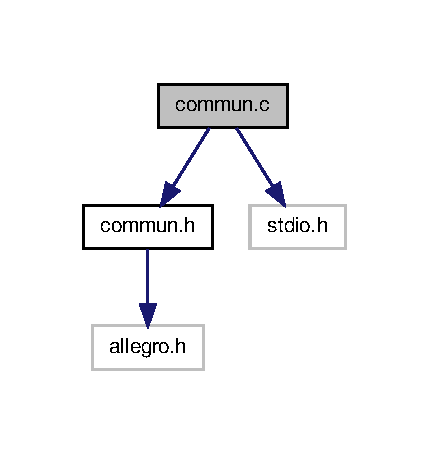
\includegraphics[width=206pt]{commun_8c__incl}
\end{center}
\end{figure}
\subsection*{Functions}
\begin{DoxyCompactItemize}
\item 
\hypertarget{commun_8c_a3c9afeeceba5da0a2457962c84e6a32b}{void \hyperlink{commun_8c_a3c9afeeceba5da0a2457962c84e6a32b}{supprimer\-\_\-piece} (int pos, \hyperlink{struct_coins}{Coins} $\ast$piece, int $\ast$nbr\-\_\-p)}\label{commun_8c_a3c9afeeceba5da0a2457962c84e6a32b}

\begin{DoxyCompactList}\small\item\em Cette fonction permet de supprimer une pièce d'un tableau de \hyperlink{struct_coins}{Coins} en prenant comme paramètre la position de la pièce à supprimer dans le tableau piece (\hyperlink{struct_coins}{Coins}) et le nombre total de pièces. \end{DoxyCompactList}\item 
\hypertarget{commun_8c_a98b3aaf8c53ced4c7ee00617437b5709}{void \hyperlink{commun_8c_a98b3aaf8c53ced4c7ee00617437b5709}{update\-\_\-pos\-\_\-coins} (\hyperlink{struct_coins}{Coins} $\ast$piece, int nbr\-\_\-p, int step)}\label{commun_8c_a98b3aaf8c53ced4c7ee00617437b5709}

\begin{DoxyCompactList}\small\item\em cette fonction permet de mettre à jour la position des pièces (\hyperlink{struct_coins}{Coins}) au fur et à mesure que la posisition du fond est modifiée. On doit faire appel à cette fonction à chaque fois que fond.\-x augmente ou diminue \end{DoxyCompactList}\item 
\hypertarget{commun_8c_a7c2650979997ebeb9f2a4d8e45a58aa2}{void \hyperlink{commun_8c_a7c2650979997ebeb9f2a4d8e45a58aa2}{init\-\_\-\-Game\-\_\-\-Over} (\hyperlink{struct_game}{Game} $\ast$game)}\label{commun_8c_a7c2650979997ebeb9f2a4d8e45a58aa2}

\begin{DoxyCompactList}\small\item\em Cette fonction permet d'initialiser la variable game de type \hyperlink{struct_game}{Game} qui est le message \hyperlink{struct_game}{Game} Over. \end{DoxyCompactList}\item 
\hypertarget{commun_8c_a6560ca25c4dad26bf465f557114cd9e1}{void \hyperlink{commun_8c_a6560ca25c4dad26bf465f557114cd9e1}{init\-\_\-\-You\-\_\-\-Win} (\hyperlink{struct_game}{Game} $\ast$win)}\label{commun_8c_a6560ca25c4dad26bf465f557114cd9e1}

\begin{DoxyCompactList}\small\item\em Cette fonction permet d'initialiser la variable win de type \hyperlink{struct_game}{Game} qui est le message You Win. \end{DoxyCompactList}\item 
void \hyperlink{commun_8c_a1f3d61077c1bb9379a7f01c8bc9a1bb1}{init\-\_\-barre\-\_\-vie} (\hyperlink{struct_barre}{Barre} $\ast$barre)
\begin{DoxyCompactList}\small\item\em Cette fonction permet d'initialiser la barre de vie (structure \hyperlink{struct_barre}{Barre}) \end{DoxyCompactList}\item 
\hypertarget{commun_8c_a20cc1e9561a79df2ab001c2036598021}{void {\bfseries init\-\_\-tete} (\hyperlink{struct_tete}{Tete} $\ast$tete)}\label{commun_8c_a20cc1e9561a79df2ab001c2036598021}

\item 
\hypertarget{commun_8c_a54d4fc08d9b64e902582638e20c39acc}{void \hyperlink{commun_8c_a54d4fc08d9b64e902582638e20c39acc}{init\-\_\-numero} (\hyperlink{struct_numero}{Numero} $\ast$numero)}\label{commun_8c_a54d4fc08d9b64e902582638e20c39acc}

\begin{DoxyCompactList}\small\item\em Cette fonction permet d'initialiser la structure \hyperlink{struct_numero}{Numero}. \end{DoxyCompactList}\item 
\hypertarget{commun_8c_ae7418c0391a1f68e6eb925ce6252b58b}{void \hyperlink{commun_8c_ae7418c0391a1f68e6eb925ce6252b58b}{destroy\-\_\-numero} (\hyperlink{struct_numero}{Numero} $\ast$numero)}\label{commun_8c_ae7418c0391a1f68e6eb925ce6252b58b}

\begin{DoxyCompactList}\small\item\em Cette fonction permet de libérer la mémoire allouée pour la structure \hyperlink{struct_numero}{Numero}. \end{DoxyCompactList}\item 
\hypertarget{commun_8c_a44437811cdbcb61edc057f27ca357e0f}{void \hyperlink{commun_8c_a44437811cdbcb61edc057f27ca357e0f}{afficher\-\_\-score} (int score, \hyperlink{struct_numero}{Numero} numero)}\label{commun_8c_a44437811cdbcb61edc057f27ca357e0f}

\begin{DoxyCompactList}\small\item\em Cette fonction permet d'afficher le score sur l'écran en utilisant les images de la structure \hyperlink{struct_numero}{Numero}. \end{DoxyCompactList}\item 
\hypertarget{commun_8c_a01023e57418ee2f80466270d13eed27b}{void \hyperlink{commun_8c_a01023e57418ee2f80466270d13eed27b}{destroy\-\_\-barre} (\hyperlink{struct_barre}{Barre} $\ast$barre)}\label{commun_8c_a01023e57418ee2f80466270d13eed27b}

\begin{DoxyCompactList}\small\item\em Cette fonction permet de libérer la mémoire allouée pour la structure \hyperlink{struct_barre}{Barre}. \end{DoxyCompactList}\item 
\hypertarget{commun_8c_a51555e8d8f6b8b988d2aea7627e99ba5}{void \hyperlink{commun_8c_a51555e8d8f6b8b988d2aea7627e99ba5}{destroy\-\_\-frog} (\hyperlink{struct_froggy}{Froggy} $\ast$frog)}\label{commun_8c_a51555e8d8f6b8b988d2aea7627e99ba5}

\begin{DoxyCompactList}\small\item\em Cette fonction permet de libérer la mémoire allouée pour la structure \hyperlink{struct_froggy}{Froggy}. \end{DoxyCompactList}\item 
\hypertarget{commun_8c_aa3947c2cfbd7fc011c4c56fb5de1ad64}{void \hyperlink{commun_8c_aa3947c2cfbd7fc011c4c56fb5de1ad64}{init\-\_\-pause} (\hyperlink{struct_pause}{Pause} $\ast$pause)}\label{commun_8c_aa3947c2cfbd7fc011c4c56fb5de1ad64}

\begin{DoxyCompactList}\small\item\em Cette fonction permet d'initialiser la structure \hyperlink{struct_pause}{Pause} (menu pause) \end{DoxyCompactList}\item 
\hypertarget{commun_8c_a66232ff660c851787839cecb2cda1288}{int \hyperlink{commun_8c_a66232ff660c851787839cecb2cda1288}{select\-\_\-next} ()}\label{commun_8c_a66232ff660c851787839cecb2cda1288}

\begin{DoxyCompactList}\small\item\em Cette fonction permet de vérifier si le curseur de la souris est pointé ou non sur le bouton next de la structure \hyperlink{struct_game}{Game}. Si c'est le cas elle retourne 1 sinon elle retourne 0. \end{DoxyCompactList}\item 
\hypertarget{commun_8c_a377375d3c30a972f57bab591a8a366ad}{int \hyperlink{commun_8c_a377375d3c30a972f57bab591a8a366ad}{pause\-\_\-curseur} ()}\label{commun_8c_a377375d3c30a972f57bab591a8a366ad}

\begin{DoxyCompactList}\small\item\em Cette fonction permet de vérifier sur quel bouton du menu \hyperlink{struct_pause}{Pause} le curseur de la souris est pointé. Si il est pointé sur le bouton \char`\"{}resume\char`\"{} elle retourne 1, si c'est sur le bouton \char`\"{}quit\char`\"{} elle retourne 2 sinon elle retourne 0. \end{DoxyCompactList}\item 
\hypertarget{commun_8c_a61ea9e7d73e9acd8b328d22508ed3fc0}{void \hyperlink{commun_8c_a61ea9e7d73e9acd8b328d22508ed3fc0}{saving} (int stage\-\_\-deverouille)}\label{commun_8c_a61ea9e7d73e9acd8b328d22508ed3fc0}

\begin{DoxyCompactList}\small\item\em Cette fonction permet une variable de type entier dans un fichier nommé \char`\"{}save.\-txt\char`\"{}. Elle crée un nouveau fichier si celui ci n'existe pas et elle écrase son ancien contenu. \end{DoxyCompactList}\item 
\hypertarget{commun_8c_aa230b82e6ddb07b5b03406c332cbec4e}{int \hyperlink{commun_8c_aa230b82e6ddb07b5b03406c332cbec4e}{loading} ()}\label{commun_8c_aa230b82e6ddb07b5b03406c332cbec4e}

\begin{DoxyCompactList}\small\item\em Cette fonction permet de charger un entier qui se trouve dans le fichier \char`\"{}save.\-txt\char`\"{} et le retourner. \end{DoxyCompactList}\item 
\hypertarget{commun_8c_a5c55e1f07b487054c01c9dff7eee8acf}{void \hyperlink{commun_8c_a5c55e1f07b487054c01c9dff7eee8acf}{conversion\-\_\-stage\-\_\-etat\-\_\-s} (int stage\-\_\-deverouille, int $\ast$etat\-\_\-s2, int $\ast$etat\-\_\-s3, int $\ast$etat\-\_\-s4)}\label{commun_8c_a5c55e1f07b487054c01c9dff7eee8acf}

\begin{DoxyCompactList}\small\item\em Cette fonction permet de convertir allant de 1 à 4 en une série d'entiers correspondant à l'état ouvert ou fermé de chaque stage. \end{DoxyCompactList}\item 
\hypertarget{commun_8c_a9bd991aefaa6ef217ad07a171b6f537e}{void \hyperlink{commun_8c_a9bd991aefaa6ef217ad07a171b6f537e}{init\-\_\-chargement} (\hyperlink{struct_chargement}{Chargement} $\ast$chargement)}\label{commun_8c_a9bd991aefaa6ef217ad07a171b6f537e}

\begin{DoxyCompactList}\small\item\em Cette fonction permet d'initialiser la structure \hyperlink{struct_chargement}{Chargement}. \end{DoxyCompactList}\item 
\hypertarget{commun_8c_a1de9d12565300dee655730ad3ba1cb7f}{void \hyperlink{commun_8c_a1de9d12565300dee655730ad3ba1cb7f}{fonction\-\_\-chargement} (int $\ast$loading\-\_\-counter, int $\ast$page, int $\ast$turn\-\_\-on\-\_\-music, \hyperlink{struct_chargement}{Chargement} chargement, \hyperlink{struct_background}{Background} curious\-\_\-froggy)}\label{commun_8c_a1de9d12565300dee655730ad3ba1cb7f}

\begin{DoxyCompactList}\small\item\em Cette fonction permet d'afficher l'animation de chargement au début du jeu. \end{DoxyCompactList}\end{DoxyCompactItemize}
\subsection*{Variables}
\begin{DoxyCompactItemize}
\item 
B\-I\-T\-M\-A\-P $\ast$ \hyperlink{commun_8c_aef1bd8d993a34eb7d4b18cf5ec1657c4}{Buffer}
\begin{DoxyCompactList}\small\item\em Ceci est la déclaration du Buffer comme étant variable globale. \end{DoxyCompactList}\end{DoxyCompactItemize}


\subsection{Detailed Description}
\begin{DoxyAuthor}{Author}
Las Vegas 
\end{DoxyAuthor}
\begin{DoxyDate}{Date}
22 Mai 2013 
\end{DoxyDate}


\subsection{Function Documentation}
\hypertarget{commun_8c_a1f3d61077c1bb9379a7f01c8bc9a1bb1}{\index{commun.\-c@{commun.\-c}!init\-\_\-barre\-\_\-vie@{init\-\_\-barre\-\_\-vie}}
\index{init\-\_\-barre\-\_\-vie@{init\-\_\-barre\-\_\-vie}!commun.c@{commun.\-c}}
\subsubsection[{init\-\_\-barre\-\_\-vie}]{\setlength{\rightskip}{0pt plus 5cm}void init\-\_\-barre\-\_\-vie (
\begin{DoxyParamCaption}
\item[{{\bf Barre} $\ast$}]{barre}
\end{DoxyParamCaption}
)}}\label{commun_8c_a1f3d61077c1bb9379a7f01c8bc9a1bb1}


Cette fonction permet d'initialiser la barre de vie (structure \hyperlink{struct_barre}{Barre}) 

Cette fonction permet d'initialiser la structure \hyperlink{struct_tete}{Tete}. 

\subsection{Variable Documentation}
\hypertarget{commun_8c_aef1bd8d993a34eb7d4b18cf5ec1657c4}{\index{commun.\-c@{commun.\-c}!Buffer@{Buffer}}
\index{Buffer@{Buffer}!commun.c@{commun.\-c}}
\subsubsection[{Buffer}]{\setlength{\rightskip}{0pt plus 5cm}B\-I\-T\-M\-A\-P $\ast$ Buffer}}\label{commun_8c_aef1bd8d993a34eb7d4b18cf5ec1657c4}


Ceci est la déclaration du Buffer comme étant variable globale. 


\begin{DoxyItemize}
\item 
\end{DoxyItemize}
\hypertarget{commun_8h}{\section{commun.\-h File Reference}
\label{commun_8h}\index{commun.\-h@{commun.\-h}}
}
{\ttfamily \#include $<$allegro.\-h$>$}\\*
Include dependency graph for commun.\-h\-:\nopagebreak
\begin{figure}[H]
\begin{center}
\leavevmode
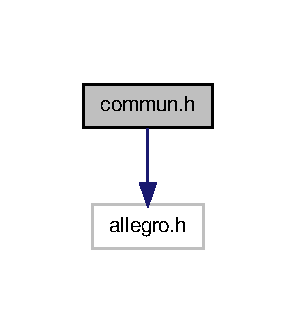
\includegraphics[width=142pt]{commun_8h__incl}
\end{center}
\end{figure}
This graph shows which files directly or indirectly include this file\-:
\nopagebreak
\begin{figure}[H]
\begin{center}
\leavevmode
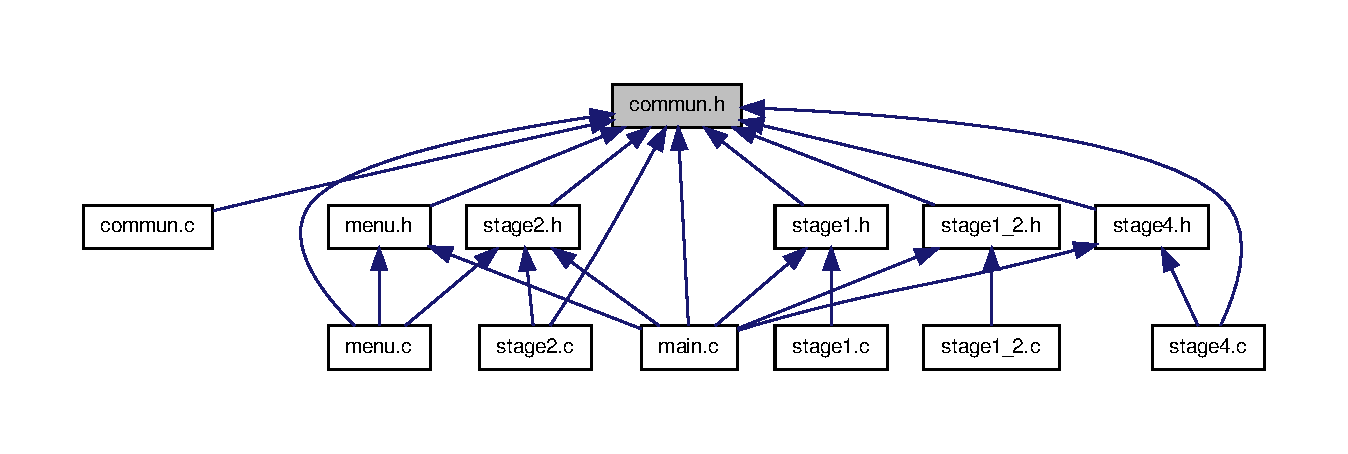
\includegraphics[width=350pt]{commun_8h__dep__incl}
\end{center}
\end{figure}
\subsection*{Data Structures}
\begin{DoxyCompactItemize}
\item 
struct \hyperlink{struct_background}{Background}
\begin{DoxyCompactList}\small\item\em x et y sont les coordonnées du fond. img contient le B\-I\-T\-M\-A\-P du fond \end{DoxyCompactList}\item 
struct \hyperlink{struct_calque}{Calque}
\begin{DoxyCompactList}\small\item\em img contient le B\-I\-T\-M\-A\-P du \hyperlink{struct_calque}{Calque} qui est qui est l'image du fond dans lequel les obstacles sont coloriés par des couleurs spécifiques (les trous en blanc de coordonnées 16777215, le plancher en bleu ciel de coordonnées 65535, la zone d'arrivée en orange de coordonnées 16850088 dans tous les stages à l'exception du stage 3 où seulement les obstacles sont coloriés en blanc de coordonnées 16777215) x est inversement proportionelle à fond.\-x. Lorsque cette dernière augmente calque.\-x diminue et inversement \end{DoxyCompactList}\item 
struct \hyperlink{struct_game}{Game}
\begin{DoxyCompactList}\small\item\em Cette structure contient les positions x et y des messages Game\-Over et You\-Win. Chacune d'eux contient deux etats mis dans 2 images dans le tableau B\-I\-T\-M\-A\-P $\ast$img\mbox{[}\mbox{]}. \end{DoxyCompactList}\item 
struct \hyperlink{struct_coins}{Coins}
\begin{DoxyCompactList}\small\item\em x et y sont les coordonnées des différentes pièces organisées dans les tableau int x\mbox{[}\mbox{]} et int y\mbox{[}\mbox{]}. img contient le B\-I\-T\-M\-A\-P du fond \end{DoxyCompactList}\item 
struct \hyperlink{struct_froggy}{Froggy}
\begin{DoxyCompactList}\small\item\em x la position de \hyperlink{struct_froggy}{Froggy} en largeur et y en hauteur. Nous avons un seul sprite \hyperlink{struct_froggy}{Froggy} dans le jeu. img est le B\-I\-T\-M\-A\-P de ce pigeon puisque il contient 7 frames donc nous avons 7 images. \end{DoxyCompactList}\item 
struct \hyperlink{struct_barre}{Barre}
\begin{DoxyCompactList}\small\item\em Celle ci est la strucuture de la barre de vie. x est la position de la \hyperlink{struct_barre}{Barre} en largeur et y en hauteur. Nous avons une seule \hyperlink{struct_barre}{Barre} de vie dans le jeu. img est le B\-I\-T\-M\-A\-P de cette \hyperlink{struct_barre}{Barre} puisque nous avons dans le jeu 6 vies donc nous avons ici 7 frames. (un pour vie = 0) \end{DoxyCompactList}\item 
struct \hyperlink{struct_tete}{Tete}
\begin{DoxyCompactList}\small\item\em Celle-\/ci est la structure de la tête de \hyperlink{struct_froggy}{Froggy} qui s'affiche en haut et à gauche de l'écran dans les stages 1,2 et 4. \end{DoxyCompactList}\item 
struct \hyperlink{struct_numero}{Numero}
\begin{DoxyCompactList}\small\item\em Cette structure contient des images de chiffres utilisées pour afficher le score. Puisque les chiffres vont de 0 à 9 donc nous avons ici 10 images. \end{DoxyCompactList}\item 
struct \hyperlink{struct_pause}{Pause}
\begin{DoxyCompactList}\small\item\em Cette structure est celle du menu de pause. Elle contient les coordonnées x et y du menu mais aussi les différents états (3 frames) \end{DoxyCompactList}\item 
struct \hyperlink{struct_chargement}{Chargement}
\begin{DoxyCompactList}\small\item\em Cette structure contient la barre de chargement du jeu avec ses 4 états d'avancement. \end{DoxyCompactList}\end{DoxyCompactItemize}
\subsection*{Macros}
\begin{DoxyCompactItemize}
\item 
\hypertarget{commun_8h_a31cf6aeb50c7069a9eecf4a5cb6b1593}{\#define {\bfseries np2}~52}\label{commun_8h_a31cf6aeb50c7069a9eecf4a5cb6b1593}

\item 
\hypertarget{commun_8h_af63e360546db8ab66144be8d3f2a4dc6}{\#define {\bfseries nbr\-\_\-piece}~34}\label{commun_8h_af63e360546db8ab66144be8d3f2a4dc6}

\item 
\hypertarget{commun_8h_ad5a96ff769b25c5d58fec87bc710c019}{\#define {\bfseries nbr\-\_\-serpent}~2}\label{commun_8h_ad5a96ff769b25c5d58fec87bc710c019}

\item 
\hypertarget{commun_8h_aaa368cdf27a0f5265ac633a3d2dae8fe}{\#define {\bfseries nbr\-\_\-reine}~3}\label{commun_8h_aaa368cdf27a0f5265ac633a3d2dae8fe}

\end{DoxyCompactItemize}
\subsection*{Functions}
\begin{DoxyCompactItemize}
\item 
\hypertarget{commun_8h_a3c9afeeceba5da0a2457962c84e6a32b}{void \hyperlink{commun_8h_a3c9afeeceba5da0a2457962c84e6a32b}{supprimer\-\_\-piece} (int pos, \hyperlink{struct_coins}{Coins} $\ast$piece, int $\ast$nbr\-\_\-p)}\label{commun_8h_a3c9afeeceba5da0a2457962c84e6a32b}

\begin{DoxyCompactList}\small\item\em Cette fonction permet de supprimer une pièce d'un tableau de \hyperlink{struct_coins}{Coins} en prenant comme paramètre la position de la pièce à supprimer dans le tableau piece (\hyperlink{struct_coins}{Coins}) et le nombre total de pièces. \end{DoxyCompactList}\item 
\hypertarget{commun_8h_a98b3aaf8c53ced4c7ee00617437b5709}{void \hyperlink{commun_8h_a98b3aaf8c53ced4c7ee00617437b5709}{update\-\_\-pos\-\_\-coins} (\hyperlink{struct_coins}{Coins} $\ast$piece, int nbr\-\_\-p, int step)}\label{commun_8h_a98b3aaf8c53ced4c7ee00617437b5709}

\begin{DoxyCompactList}\small\item\em cette fonction permet de mettre à jour la position des pièces (\hyperlink{struct_coins}{Coins}) au fur et à mesure que la posisition du fond est modifiée. On doit faire appel à cette fonction à chaque fois que fond.\-x augmente ou diminue \end{DoxyCompactList}\item 
\hypertarget{commun_8h_a7c2650979997ebeb9f2a4d8e45a58aa2}{void \hyperlink{commun_8h_a7c2650979997ebeb9f2a4d8e45a58aa2}{init\-\_\-\-Game\-\_\-\-Over} (\hyperlink{struct_game}{Game} $\ast$game)}\label{commun_8h_a7c2650979997ebeb9f2a4d8e45a58aa2}

\begin{DoxyCompactList}\small\item\em Cette fonction permet d'initialiser la variable game de type \hyperlink{struct_game}{Game} qui est le message \hyperlink{struct_game}{Game} Over. \end{DoxyCompactList}\item 
\hypertarget{commun_8h_a6560ca25c4dad26bf465f557114cd9e1}{void \hyperlink{commun_8h_a6560ca25c4dad26bf465f557114cd9e1}{init\-\_\-\-You\-\_\-\-Win} (\hyperlink{struct_game}{Game} $\ast$win)}\label{commun_8h_a6560ca25c4dad26bf465f557114cd9e1}

\begin{DoxyCompactList}\small\item\em Cette fonction permet d'initialiser la variable win de type \hyperlink{struct_game}{Game} qui est le message You Win. \end{DoxyCompactList}\item 
void \hyperlink{commun_8h_a1f3d61077c1bb9379a7f01c8bc9a1bb1}{init\-\_\-barre\-\_\-vie} (\hyperlink{struct_barre}{Barre} $\ast$barre)
\begin{DoxyCompactList}\small\item\em Cette fonction permet d'initialiser la barre de vie (structure \hyperlink{struct_barre}{Barre}) \end{DoxyCompactList}\item 
\hypertarget{commun_8h_a20cc1e9561a79df2ab001c2036598021}{void {\bfseries init\-\_\-tete} (\hyperlink{struct_tete}{Tete} $\ast$tete)}\label{commun_8h_a20cc1e9561a79df2ab001c2036598021}

\item 
\hypertarget{commun_8h_a54d4fc08d9b64e902582638e20c39acc}{void \hyperlink{commun_8h_a54d4fc08d9b64e902582638e20c39acc}{init\-\_\-numero} (\hyperlink{struct_numero}{Numero} $\ast$numero)}\label{commun_8h_a54d4fc08d9b64e902582638e20c39acc}

\begin{DoxyCompactList}\small\item\em Cette fonction permet d'initialiser la structure \hyperlink{struct_numero}{Numero}. \end{DoxyCompactList}\item 
\hypertarget{commun_8h_ae7418c0391a1f68e6eb925ce6252b58b}{void \hyperlink{commun_8h_ae7418c0391a1f68e6eb925ce6252b58b}{destroy\-\_\-numero} (\hyperlink{struct_numero}{Numero} $\ast$numero)}\label{commun_8h_ae7418c0391a1f68e6eb925ce6252b58b}

\begin{DoxyCompactList}\small\item\em Cette fonction permet de libérer la mémoire allouée pour la structure \hyperlink{struct_numero}{Numero}. \end{DoxyCompactList}\item 
\hypertarget{commun_8h_a44437811cdbcb61edc057f27ca357e0f}{void \hyperlink{commun_8h_a44437811cdbcb61edc057f27ca357e0f}{afficher\-\_\-score} (int score, \hyperlink{struct_numero}{Numero} numero)}\label{commun_8h_a44437811cdbcb61edc057f27ca357e0f}

\begin{DoxyCompactList}\small\item\em Cette fonction permet d'afficher le score sur l'écran en utilisant les images de la structure \hyperlink{struct_numero}{Numero}. \end{DoxyCompactList}\item 
\hypertarget{commun_8h_a01023e57418ee2f80466270d13eed27b}{void \hyperlink{commun_8h_a01023e57418ee2f80466270d13eed27b}{destroy\-\_\-barre} (\hyperlink{struct_barre}{Barre} $\ast$barre)}\label{commun_8h_a01023e57418ee2f80466270d13eed27b}

\begin{DoxyCompactList}\small\item\em Cette fonction permet de libérer la mémoire allouée pour la structure \hyperlink{struct_barre}{Barre}. \end{DoxyCompactList}\item 
\hypertarget{commun_8h_a51555e8d8f6b8b988d2aea7627e99ba5}{void \hyperlink{commun_8h_a51555e8d8f6b8b988d2aea7627e99ba5}{destroy\-\_\-frog} (\hyperlink{struct_froggy}{Froggy} $\ast$frog)}\label{commun_8h_a51555e8d8f6b8b988d2aea7627e99ba5}

\begin{DoxyCompactList}\small\item\em Cette fonction permet de libérer la mémoire allouée pour la structure \hyperlink{struct_froggy}{Froggy}. \end{DoxyCompactList}\item 
\hypertarget{commun_8h_aa3947c2cfbd7fc011c4c56fb5de1ad64}{void \hyperlink{commun_8h_aa3947c2cfbd7fc011c4c56fb5de1ad64}{init\-\_\-pause} (\hyperlink{struct_pause}{Pause} $\ast$pause)}\label{commun_8h_aa3947c2cfbd7fc011c4c56fb5de1ad64}

\begin{DoxyCompactList}\small\item\em Cette fonction permet d'initialiser la structure \hyperlink{struct_pause}{Pause} (menu pause) \end{DoxyCompactList}\item 
\hypertarget{commun_8h_a66232ff660c851787839cecb2cda1288}{int \hyperlink{commun_8h_a66232ff660c851787839cecb2cda1288}{select\-\_\-next} ()}\label{commun_8h_a66232ff660c851787839cecb2cda1288}

\begin{DoxyCompactList}\small\item\em Cette fonction permet de vérifier si le curseur de la souris est pointé ou non sur le bouton next de la structure \hyperlink{struct_game}{Game}. Si c'est le cas elle retourne 1 sinon elle retourne 0. \end{DoxyCompactList}\item 
\hypertarget{commun_8h_a377375d3c30a972f57bab591a8a366ad}{int \hyperlink{commun_8h_a377375d3c30a972f57bab591a8a366ad}{pause\-\_\-curseur} ()}\label{commun_8h_a377375d3c30a972f57bab591a8a366ad}

\begin{DoxyCompactList}\small\item\em Cette fonction permet de vérifier sur quel bouton du menu \hyperlink{struct_pause}{Pause} le curseur de la souris est pointé. Si il est pointé sur le bouton \char`\"{}resume\char`\"{} elle retourne 1, si c'est sur le bouton \char`\"{}quit\char`\"{} elle retourne 2 sinon elle retourne 0. \end{DoxyCompactList}\item 
\hypertarget{commun_8h_a61ea9e7d73e9acd8b328d22508ed3fc0}{void \hyperlink{commun_8h_a61ea9e7d73e9acd8b328d22508ed3fc0}{saving} (int stage\-\_\-deverouille)}\label{commun_8h_a61ea9e7d73e9acd8b328d22508ed3fc0}

\begin{DoxyCompactList}\small\item\em Cette fonction permet une variable de type entier dans un fichier nommé \char`\"{}save.\-txt\char`\"{}. Elle crée un nouveau fichier si celui ci n'existe pas et elle écrase son ancien contenu. \end{DoxyCompactList}\item 
\hypertarget{commun_8h_aa230b82e6ddb07b5b03406c332cbec4e}{int \hyperlink{commun_8h_aa230b82e6ddb07b5b03406c332cbec4e}{loading} ()}\label{commun_8h_aa230b82e6ddb07b5b03406c332cbec4e}

\begin{DoxyCompactList}\small\item\em Cette fonction permet de charger un entier qui se trouve dans le fichier \char`\"{}save.\-txt\char`\"{} et le retourner. \end{DoxyCompactList}\item 
\hypertarget{commun_8h_a5c55e1f07b487054c01c9dff7eee8acf}{void \hyperlink{commun_8h_a5c55e1f07b487054c01c9dff7eee8acf}{conversion\-\_\-stage\-\_\-etat\-\_\-s} (int stage\-\_\-deverouille, int $\ast$etat\-\_\-s2, int $\ast$etat\-\_\-s3, int $\ast$etat\-\_\-s4)}\label{commun_8h_a5c55e1f07b487054c01c9dff7eee8acf}

\begin{DoxyCompactList}\small\item\em Cette fonction permet de convertir allant de 1 à 4 en une série d'entiers correspondant à l'état ouvert ou fermé de chaque stage. \end{DoxyCompactList}\item 
\hypertarget{commun_8h_a9bd991aefaa6ef217ad07a171b6f537e}{void \hyperlink{commun_8h_a9bd991aefaa6ef217ad07a171b6f537e}{init\-\_\-chargement} (\hyperlink{struct_chargement}{Chargement} $\ast$chargement)}\label{commun_8h_a9bd991aefaa6ef217ad07a171b6f537e}

\begin{DoxyCompactList}\small\item\em Cette fonction permet d'initialiser la structure \hyperlink{struct_chargement}{Chargement}. \end{DoxyCompactList}\item 
\hypertarget{commun_8h_a1de9d12565300dee655730ad3ba1cb7f}{void \hyperlink{commun_8h_a1de9d12565300dee655730ad3ba1cb7f}{fonction\-\_\-chargement} (int $\ast$loading\-\_\-counter, int $\ast$page, int $\ast$turn\-\_\-on\-\_\-music, \hyperlink{struct_chargement}{Chargement} chargement, \hyperlink{struct_background}{Background} curious\-\_\-froggy)}\label{commun_8h_a1de9d12565300dee655730ad3ba1cb7f}

\begin{DoxyCompactList}\small\item\em Cette fonction permet d'afficher l'animation de chargement au début du jeu. \end{DoxyCompactList}\end{DoxyCompactItemize}
\subsection*{Variables}
\begin{DoxyCompactItemize}
\item 
B\-I\-T\-M\-A\-P $\ast$ \hyperlink{commun_8h_a700c2011fa3d781837c4d795a70c7c9d}{Buffer}
\begin{DoxyCompactList}\small\item\em Ceci est la déclaration du Buffer comme étant variable globale. \end{DoxyCompactList}\end{DoxyCompactItemize}


\subsection{Detailed Description}
\begin{DoxyAuthor}{Author}
Las Vegas 
\end{DoxyAuthor}
\begin{DoxyDate}{Date}
22 Mai 2013 
\end{DoxyDate}


\subsection{Function Documentation}
\hypertarget{commun_8h_a1f3d61077c1bb9379a7f01c8bc9a1bb1}{\index{commun.\-h@{commun.\-h}!init\-\_\-barre\-\_\-vie@{init\-\_\-barre\-\_\-vie}}
\index{init\-\_\-barre\-\_\-vie@{init\-\_\-barre\-\_\-vie}!commun.h@{commun.\-h}}
\subsubsection[{init\-\_\-barre\-\_\-vie}]{\setlength{\rightskip}{0pt plus 5cm}void init\-\_\-barre\-\_\-vie (
\begin{DoxyParamCaption}
\item[{{\bf Barre} $\ast$}]{barre}
\end{DoxyParamCaption}
)}}\label{commun_8h_a1f3d61077c1bb9379a7f01c8bc9a1bb1}


Cette fonction permet d'initialiser la barre de vie (structure \hyperlink{struct_barre}{Barre}) 

Cette fonction permet d'initialiser la structure \hyperlink{struct_tete}{Tete}. 

\subsection{Variable Documentation}
\hypertarget{commun_8h_a700c2011fa3d781837c4d795a70c7c9d}{\index{commun.\-h@{commun.\-h}!Buffer@{Buffer}}
\index{Buffer@{Buffer}!commun.h@{commun.\-h}}
\subsubsection[{Buffer}]{\setlength{\rightskip}{0pt plus 5cm}B\-I\-T\-M\-A\-P$\ast$ Buffer}}\label{commun_8h_a700c2011fa3d781837c4d795a70c7c9d}


Ceci est la déclaration du Buffer comme étant variable globale. 


\begin{DoxyItemize}
\item 
\end{DoxyItemize}
\hypertarget{main_8c}{\section{main.\-c File Reference}
\label{main_8c}\index{main.\-c@{main.\-c}}
}
{\ttfamily \#include $<$allegro.\-h$>$}\\*
{\ttfamily \#include $<$apeg.\-h$>$}\\*
{\ttfamily \#include \char`\"{}menu.\-h\char`\"{}}\\*
{\ttfamily \#include \char`\"{}commun.\-h\char`\"{}}\\*
{\ttfamily \#include \char`\"{}stage2.\-h\char`\"{}}\\*
{\ttfamily \#include \char`\"{}stage1.\-h\char`\"{}}\\*
{\ttfamily \#include \char`\"{}stage1\-\_\-2.\-h\char`\"{}}\\*
{\ttfamily \#include \char`\"{}stage4.\-h\char`\"{}}\\*
Include dependency graph for main.\-c\-:
\nopagebreak
\begin{figure}[H]
\begin{center}
\leavevmode
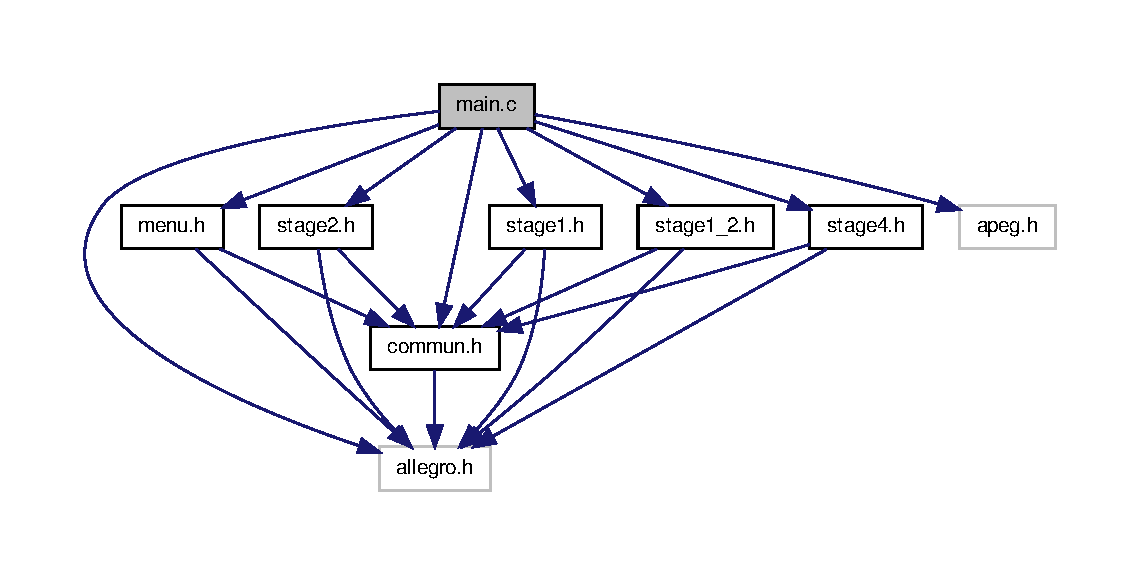
\includegraphics[width=350pt]{main_8c__incl}
\end{center}
\end{figure}
\subsection*{Functions}
\begin{DoxyCompactItemize}
\item 
\hypertarget{main_8c_ae66f6b31b5ad750f1fe042a706a4e3d4}{int {\bfseries main} ()}\label{main_8c_ae66f6b31b5ad750f1fe042a706a4e3d4}

\end{DoxyCompactItemize}
\subsection*{Variables}
\begin{DoxyCompactItemize}
\item 
B\-I\-T\-M\-A\-P $\ast$ \hyperlink{main_8c_a700c2011fa3d781837c4d795a70c7c9d}{Buffer}
\begin{DoxyCompactList}\small\item\em Ceci est la déclaration du Buffer comme étant variable globale. \end{DoxyCompactList}\end{DoxyCompactItemize}


\subsection{Detailed Description}
\begin{DoxyAuthor}{Author}
Las Vegas 
\end{DoxyAuthor}
\begin{DoxyDate}{Date}
22 Mai 2013 
\end{DoxyDate}


\subsection{Variable Documentation}
\hypertarget{main_8c_a700c2011fa3d781837c4d795a70c7c9d}{\index{main.\-c@{main.\-c}!Buffer@{Buffer}}
\index{Buffer@{Buffer}!main.c@{main.\-c}}
\subsubsection[{Buffer}]{\setlength{\rightskip}{0pt plus 5cm}B\-I\-T\-M\-A\-P$\ast$ Buffer}}\label{main_8c_a700c2011fa3d781837c4d795a70c7c9d}


Ceci est la déclaration du Buffer comme étant variable globale. 


\begin{DoxyItemize}
\item 
\end{DoxyItemize}
\hypertarget{menu_8c}{\section{menu.\-c File Reference}
\label{menu_8c}\index{menu.\-c@{menu.\-c}}
}
{\ttfamily \#include \char`\"{}menu.\-h\char`\"{}}\\*
{\ttfamily \#include \char`\"{}commun.\-h\char`\"{}}\\*
{\ttfamily \#include \char`\"{}stage2.\-h\char`\"{}}\\*
Include dependency graph for menu.\-c\-:
\nopagebreak
\begin{figure}[H]
\begin{center}
\leavevmode
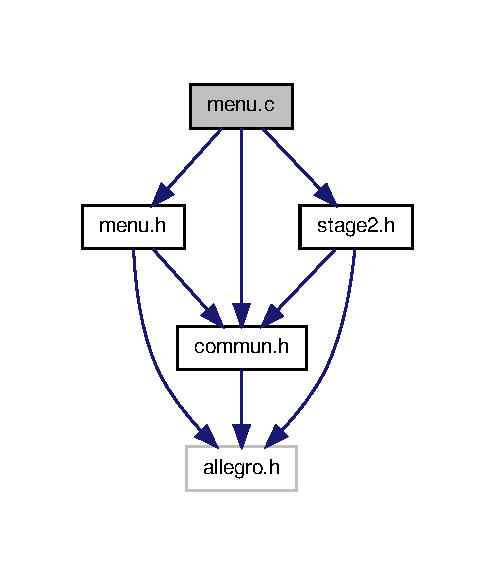
\includegraphics[width=238pt]{menu_8c__incl}
\end{center}
\end{figure}
\subsection*{Functions}
\begin{DoxyCompactItemize}
\item 
\hypertarget{menu_8c_a599934adf271c51c067770688c25aedb}{void \hyperlink{menu_8c_a599934adf271c51c067770688c25aedb}{init\-\_\-fond\-\_\-menu} (\hyperlink{struct_background}{Background} $\ast$fond)}\label{menu_8c_a599934adf271c51c067770688c25aedb}

\begin{DoxyCompactList}\small\item\em cette fonction permet d'initialiser le fond du menu \end{DoxyCompactList}\item 
\hypertarget{menu_8c_a2d4a1303a1a1a59a3fa2bda3e676e459}{void \hyperlink{menu_8c_a2d4a1303a1a1a59a3fa2bda3e676e459}{init\-\_\-menu1} (\hyperlink{structbouton}{bouton} $\ast$exit, \hyperlink{structbouton}{bouton} $\ast$help, \hyperlink{structbouton}{bouton} $\ast$play, \hyperlink{structbouton}{bouton} $\ast$son, \hyperlink{structbouton}{bouton} $\ast$son\-\_\-coupe)}\label{menu_8c_a2d4a1303a1a1a59a3fa2bda3e676e459}

\begin{DoxyCompactList}\small\item\em Cette fonction permet d'initialiser les boutons du menu 1. \end{DoxyCompactList}\item 
\hypertarget{menu_8c_a7e3d87fbff22d0836999aaf16cefce5c}{void \hyperlink{menu_8c_a7e3d87fbff22d0836999aaf16cefce5c}{init\-\_\-menu2} (\hyperlink{structicone__stage1}{icone\-\_\-stage1} $\ast$s1, \hyperlink{structicone__stage2}{icone\-\_\-stage2} $\ast$s2, \hyperlink{structicone__stage3}{icone\-\_\-stage3} $\ast$s3, \hyperlink{structicone__stage4}{icone\-\_\-stage4} $\ast$s4)}\label{menu_8c_a7e3d87fbff22d0836999aaf16cefce5c}

\begin{DoxyCompactList}\small\item\em Cette fonction permet d'initialiser les icônes du menu 2. \end{DoxyCompactList}\item 
\hypertarget{menu_8c_ae5e02e8e8c8ff7138a9dea9e7f3cd773}{void \hyperlink{menu_8c_ae5e02e8e8c8ff7138a9dea9e7f3cd773}{init\-\_\-bouton\-\_\-prec} (\hyperlink{structbouton}{bouton} $\ast$prec)}\label{menu_8c_ae5e02e8e8c8ff7138a9dea9e7f3cd773}

\begin{DoxyCompactList}\small\item\em Cette fonction permet d'initialiser le bouton précédent (prec) qui apparait dans chacun des menus 1, 2 et help. \end{DoxyCompactList}\item 
\hypertarget{menu_8c_a11ab651a6b829e622d2bc7317f8053ee}{void \hyperlink{menu_8c_a11ab651a6b829e622d2bc7317f8053ee}{etat\-\_\-bouton\-\_\-prec} (int $\ast$b\-\_\-prec)}\label{menu_8c_a11ab651a6b829e622d2bc7317f8053ee}

\begin{DoxyCompactList}\small\item\em Cette fonction permet de vérifier si le curseur est pointé ou non sur le bouton précédent (prec) Elle retourne 1 si le curseur est pointé sur le bouton, 2 si en plus la touche gauche de la souris sinon elle retourne 0. \end{DoxyCompactList}\item 
\hypertarget{menu_8c_acf717aebdff0be29c72cfa44d5ca80ed}{void \hyperlink{menu_8c_acf717aebdff0be29c72cfa44d5ca80ed}{etat\-\_\-bouton} (int $\ast$b\-\_\-play, int $\ast$b\-\_\-exit, int $\ast$b\-\_\-help, int $\ast$b\-\_\-son)}\label{menu_8c_acf717aebdff0be29c72cfa44d5ca80ed}

\begin{DoxyCompactList}\small\item\em Cette fonction permet de vérifier si le curseur est pointé ou non sur l'un des boutons du menu 1. Chaque paramètre reçoit 1 si le curseur est pointé sur le bouton, 2 si en plus la touche gauche de la souris sinon il prend la valeur de 0. \end{DoxyCompactList}\item 
\hypertarget{menu_8c_a3ebb49f8f9d68cf8afef90fbcf0a9af3}{void \hyperlink{menu_8c_a3ebb49f8f9d68cf8afef90fbcf0a9af3}{blit\-\_\-boutons} (int b\-\_\-play, int b\-\_\-exit, int b\-\_\-help, int b\-\_\-son, \hyperlink{structbouton}{bouton} exit, \hyperlink{structbouton}{bouton} help, \hyperlink{structbouton}{bouton} play, \hyperlink{structbouton}{bouton} son, \hyperlink{structbouton}{bouton} son\-\_\-coupe, int sound\-\_\-off)}\label{menu_8c_a3ebb49f8f9d68cf8afef90fbcf0a9af3}

\begin{DoxyCompactList}\small\item\em Cette fonction permet les boutons du menu 1 en fonction de leur état. \end{DoxyCompactList}\item 
\hypertarget{menu_8c_a0b78f1388066640830d349a6ab2f08f6}{void \hyperlink{menu_8c_a0b78f1388066640830d349a6ab2f08f6}{destroy\-\_\-boutons} (\hyperlink{structbouton}{bouton} $\ast$exit, \hyperlink{structbouton}{bouton} $\ast$help, \hyperlink{structbouton}{bouton} $\ast$play, \hyperlink{structbouton}{bouton} $\ast$son)}\label{menu_8c_a0b78f1388066640830d349a6ab2f08f6}

\begin{DoxyCompactList}\small\item\em Cette fonction permet de libérer la mémoire allouée pour les boutons du menu 1 qui sont de type Bouton. \end{DoxyCompactList}\item 
\hypertarget{menu_8c_a4da3c53aeeb42c0f05cd74a5aeb8c9dc}{void \hyperlink{menu_8c_a4da3c53aeeb42c0f05cd74a5aeb8c9dc}{destroy\-\_\-icones} (\hyperlink{structicone__stage1}{icone\-\_\-stage1} $\ast$s1, \hyperlink{structicone__stage2}{icone\-\_\-stage2} $\ast$s2, \hyperlink{structicone__stage3}{icone\-\_\-stage3} $\ast$s3, \hyperlink{structicone__stage4}{icone\-\_\-stage4} $\ast$s4)}\label{menu_8c_a4da3c53aeeb42c0f05cd74a5aeb8c9dc}

\begin{DoxyCompactList}\small\item\em Cette fonction permet de libérer la mémoire allouée pour les icônes du menu 2 qui sont de type \hyperlink{structicone__stage2}{icone\-\_\-stage2}. \end{DoxyCompactList}\item 
\hypertarget{menu_8c_a3a55ee75b3fdef8a9982eba0898f496c}{void \hyperlink{menu_8c_a3a55ee75b3fdef8a9982eba0898f496c}{blit\-\_\-icones} (int etat\-\_\-s2, int etat\-\_\-s3, int etat\-\_\-s4, \hyperlink{structicone__stage1}{icone\-\_\-stage1} s1, \hyperlink{structicone__stage2}{icone\-\_\-stage2} s2, \hyperlink{structicone__stage3}{icone\-\_\-stage3} s3, \hyperlink{structicone__stage4}{icone\-\_\-stage4} s4)}\label{menu_8c_a3a55ee75b3fdef8a9982eba0898f496c}

\begin{DoxyCompactList}\small\item\em Cette fonction permet les icônes du menu 2 en fonction de leur état. \end{DoxyCompactList}\item 
\hypertarget{menu_8c_ab7e8edea86ab2307d0bcc707e515a3af}{int \hyperlink{menu_8c_ab7e8edea86ab2307d0bcc707e515a3af}{select\-\_\-stage} ()}\label{menu_8c_ab7e8edea86ab2307d0bcc707e515a3af}

\begin{DoxyCompactList}\small\item\em Cette fonction permet de vérifier si le curseur est pointé ou non sur l'une des icônes du menu 2. Elle retourne 1 si le curseur est pointé sur l'icône du stage 1, 2 pour le stage 2, 3 pour le stage 3 et 4 pour le stage 4. \end{DoxyCompactList}\item 
\hypertarget{menu_8c_a3a09b0f3e820fc265bd8a80e596bd733}{void \hyperlink{menu_8c_a3a09b0f3e820fc265bd8a80e596bd733}{init\-\_\-menu\-\_\-help} (\hyperlink{struct_background}{Background} $\ast$menu\-\_\-help)}\label{menu_8c_a3a09b0f3e820fc265bd8a80e596bd733}

\begin{DoxyCompactList}\small\item\em Cette fonction permet d'initialiser le menu help. \end{DoxyCompactList}\item 
\hypertarget{menu_8c_a449b7998c1f0ae5c38e6f0e028939013}{void \hyperlink{menu_8c_a449b7998c1f0ae5c38e6f0e028939013}{fonction\-\_\-menu} (int $\ast$continuer, \hyperlink{struct_background}{Background} fond\-\_\-menu, \hyperlink{struct_background}{Background} menu\-\_\-help, int $\ast$page, \hyperlink{structbouton}{bouton} exit, \hyperlink{structbouton}{bouton} help, \hyperlink{structbouton}{bouton} play, \hyperlink{structbouton}{bouton} son, \hyperlink{structbouton}{bouton} prec, \hyperlink{structicone__stage1}{icone\-\_\-stage1} s1, \hyperlink{structicone__stage2}{icone\-\_\-stage2} s2, \hyperlink{structicone__stage3}{icone\-\_\-stage3} s3, \hyperlink{structicone__stage4}{icone\-\_\-stage4} s4, B\-I\-T\-M\-A\-P $\ast$Cursor, int $\ast$b\-\_\-play, int $\ast$b\-\_\-exit, int $\ast$b\-\_\-help, int $\ast$b\-\_\-son, int $\ast$menu, int $\ast$etat\-\_\-s2, int $\ast$etat\-\_\-s3, int $\ast$etat\-\_\-s4, int $\ast$b\-\_\-prec, int stage\-\_\-deverouille, int $\ast$turn\-\_\-on\-\_\-music, \hyperlink{structbouton}{bouton} son\-\_\-coupe, int $\ast$sound\-\_\-off, int $\ast$bloquer\-\_\-click, int $\ast$click\-\_\-counter)}\label{menu_8c_a449b7998c1f0ae5c38e6f0e028939013}

\begin{DoxyCompactList}\small\item\em Cette fonction permet de faire appel aux fonctions du menu. \end{DoxyCompactList}\end{DoxyCompactItemize}
\subsection*{Variables}
\begin{DoxyCompactItemize}
\item 
B\-I\-T\-M\-A\-P $\ast$ \hyperlink{menu_8c_a700c2011fa3d781837c4d795a70c7c9d}{Buffer}
\begin{DoxyCompactList}\small\item\em Ceci est la déclaration du Buffer comme étant variable globale. \end{DoxyCompactList}\end{DoxyCompactItemize}


\subsection{Detailed Description}
\begin{DoxyAuthor}{Author}
Las Vegas 
\end{DoxyAuthor}
\begin{DoxyDate}{Date}
22 Mai 2013 
\end{DoxyDate}


\subsection{Variable Documentation}
\hypertarget{menu_8c_a700c2011fa3d781837c4d795a70c7c9d}{\index{menu.\-c@{menu.\-c}!Buffer@{Buffer}}
\index{Buffer@{Buffer}!menu.c@{menu.\-c}}
\subsubsection[{Buffer}]{\setlength{\rightskip}{0pt plus 5cm}B\-I\-T\-M\-A\-P$\ast$ Buffer}}\label{menu_8c_a700c2011fa3d781837c4d795a70c7c9d}


Ceci est la déclaration du Buffer comme étant variable globale. 


\begin{DoxyItemize}
\item 
\end{DoxyItemize}
\hypertarget{menu_8h}{\section{menu.\-h File Reference}
\label{menu_8h}\index{menu.\-h@{menu.\-h}}
}
{\ttfamily \#include $<$allegro.\-h$>$}\\*
{\ttfamily \#include \char`\"{}commun.\-h\char`\"{}}\\*
Include dependency graph for menu.\-h\-:
\nopagebreak
\begin{figure}[H]
\begin{center}
\leavevmode
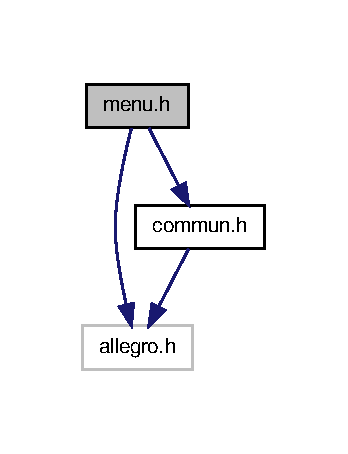
\includegraphics[width=167pt]{menu_8h__incl}
\end{center}
\end{figure}
This graph shows which files directly or indirectly include this file\-:
\nopagebreak
\begin{figure}[H]
\begin{center}
\leavevmode
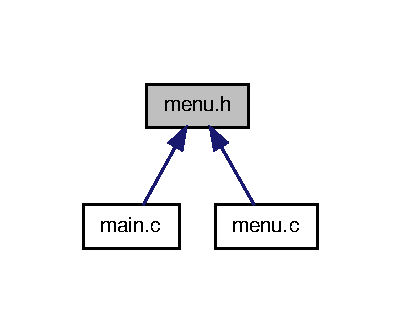
\includegraphics[width=192pt]{menu_8h__dep__incl}
\end{center}
\end{figure}
\subsection*{Data Structures}
\begin{DoxyCompactItemize}
\item 
struct \hyperlink{structbouton}{bouton}
\begin{DoxyCompactList}\small\item\em Ceci est la structure d'un bouton qui doit apparaitre dans le menu. Elle contient les coordonnées du bouton et ses différents états (3 images) \end{DoxyCompactList}\item 
struct \hyperlink{structicone__stage1}{icone\-\_\-stage1}
\begin{DoxyCompactList}\small\item\em Ceci est la structure d'une icône du stage 1 qui doit apparaitre dans le menu. Elle contient les coordonnées de l'icône. \end{DoxyCompactList}\item 
struct \hyperlink{structicone__stage2}{icone\-\_\-stage2}
\begin{DoxyCompactList}\small\item\em Ceci est la structure d'une icône du stage 2 qui doit apparaitre dans le menu. Elle contient les coordonnées de l'icône et ses différents états (2 images) verouillé ou ouvert. \end{DoxyCompactList}\item 
struct \hyperlink{structicone__stage3}{icone\-\_\-stage3}
\begin{DoxyCompactList}\small\item\em Ceci est la structure d'une icône du stage 3 qui doit apparaitre dans le menu. Elle contient les coordonnées de l'icône et ses différents états (2 images) verouillé ou ouvert. \end{DoxyCompactList}\item 
struct \hyperlink{structicone__stage4}{icone\-\_\-stage4}
\begin{DoxyCompactList}\small\item\em Ceci est la structure d'une icône du stage 4 qui doit apparaitre dans le menu. Elle contient les coordonnées de l'icône et ses différents états (2 images) verouillé ou ouvert. \end{DoxyCompactList}\end{DoxyCompactItemize}
\subsection*{Functions}
\begin{DoxyCompactItemize}
\item 
\hypertarget{menu_8h_a599934adf271c51c067770688c25aedb}{void \hyperlink{menu_8h_a599934adf271c51c067770688c25aedb}{init\-\_\-fond\-\_\-menu} (\hyperlink{struct_background}{Background} $\ast$fond)}\label{menu_8h_a599934adf271c51c067770688c25aedb}

\begin{DoxyCompactList}\small\item\em cette fonction permet d'initialiser le fond du menu \end{DoxyCompactList}\item 
\hypertarget{menu_8h_a2d4a1303a1a1a59a3fa2bda3e676e459}{void \hyperlink{menu_8h_a2d4a1303a1a1a59a3fa2bda3e676e459}{init\-\_\-menu1} (\hyperlink{structbouton}{bouton} $\ast$exit, \hyperlink{structbouton}{bouton} $\ast$help, \hyperlink{structbouton}{bouton} $\ast$play, \hyperlink{structbouton}{bouton} $\ast$son, \hyperlink{structbouton}{bouton} $\ast$son\-\_\-coupe)}\label{menu_8h_a2d4a1303a1a1a59a3fa2bda3e676e459}

\begin{DoxyCompactList}\small\item\em Cette fonction permet d'initialiser les boutons du menu 1. \end{DoxyCompactList}\item 
\hypertarget{menu_8h_a7e3d87fbff22d0836999aaf16cefce5c}{void \hyperlink{menu_8h_a7e3d87fbff22d0836999aaf16cefce5c}{init\-\_\-menu2} (\hyperlink{structicone__stage1}{icone\-\_\-stage1} $\ast$s1, \hyperlink{structicone__stage2}{icone\-\_\-stage2} $\ast$s2, \hyperlink{structicone__stage3}{icone\-\_\-stage3} $\ast$s3, \hyperlink{structicone__stage4}{icone\-\_\-stage4} $\ast$s4)}\label{menu_8h_a7e3d87fbff22d0836999aaf16cefce5c}

\begin{DoxyCompactList}\small\item\em Cette fonction permet d'initialiser les icônes du menu 2. \end{DoxyCompactList}\item 
\hypertarget{menu_8h_ae5e02e8e8c8ff7138a9dea9e7f3cd773}{void \hyperlink{menu_8h_ae5e02e8e8c8ff7138a9dea9e7f3cd773}{init\-\_\-bouton\-\_\-prec} (\hyperlink{structbouton}{bouton} $\ast$prec)}\label{menu_8h_ae5e02e8e8c8ff7138a9dea9e7f3cd773}

\begin{DoxyCompactList}\small\item\em Cette fonction permet d'initialiser le bouton précédent (prec) qui apparait dans chacun des menus 1, 2 et help. \end{DoxyCompactList}\item 
\hypertarget{menu_8h_a11ab651a6b829e622d2bc7317f8053ee}{void \hyperlink{menu_8h_a11ab651a6b829e622d2bc7317f8053ee}{etat\-\_\-bouton\-\_\-prec} (int $\ast$b\-\_\-prec)}\label{menu_8h_a11ab651a6b829e622d2bc7317f8053ee}

\begin{DoxyCompactList}\small\item\em Cette fonction permet de vérifier si le curseur est pointé ou non sur le bouton précédent (prec) Elle retourne 1 si le curseur est pointé sur le bouton, 2 si en plus la touche gauche de la souris sinon elle retourne 0. \end{DoxyCompactList}\item 
\hypertarget{menu_8h_acf717aebdff0be29c72cfa44d5ca80ed}{void \hyperlink{menu_8h_acf717aebdff0be29c72cfa44d5ca80ed}{etat\-\_\-bouton} (int $\ast$b\-\_\-play, int $\ast$b\-\_\-exit, int $\ast$b\-\_\-help, int $\ast$b\-\_\-son)}\label{menu_8h_acf717aebdff0be29c72cfa44d5ca80ed}

\begin{DoxyCompactList}\small\item\em Cette fonction permet de vérifier si le curseur est pointé ou non sur l'un des boutons du menu 1. Chaque paramètre reçoit 1 si le curseur est pointé sur le bouton, 2 si en plus la touche gauche de la souris sinon il prend la valeur de 0. \end{DoxyCompactList}\item 
\hypertarget{menu_8h_a3ebb49f8f9d68cf8afef90fbcf0a9af3}{void \hyperlink{menu_8h_a3ebb49f8f9d68cf8afef90fbcf0a9af3}{blit\-\_\-boutons} (int b\-\_\-play, int b\-\_\-exit, int b\-\_\-help, int b\-\_\-son, \hyperlink{structbouton}{bouton} exit, \hyperlink{structbouton}{bouton} help, \hyperlink{structbouton}{bouton} play, \hyperlink{structbouton}{bouton} son, \hyperlink{structbouton}{bouton} son\-\_\-coupe, int sound\-\_\-off)}\label{menu_8h_a3ebb49f8f9d68cf8afef90fbcf0a9af3}

\begin{DoxyCompactList}\small\item\em Cette fonction permet les boutons du menu 1 en fonction de leur état. \end{DoxyCompactList}\item 
\hypertarget{menu_8h_a0b78f1388066640830d349a6ab2f08f6}{void \hyperlink{menu_8h_a0b78f1388066640830d349a6ab2f08f6}{destroy\-\_\-boutons} (\hyperlink{structbouton}{bouton} $\ast$exit, \hyperlink{structbouton}{bouton} $\ast$help, \hyperlink{structbouton}{bouton} $\ast$play, \hyperlink{structbouton}{bouton} $\ast$son)}\label{menu_8h_a0b78f1388066640830d349a6ab2f08f6}

\begin{DoxyCompactList}\small\item\em Cette fonction permet de libérer la mémoire allouée pour les boutons du menu 1 qui sont de type Bouton. \end{DoxyCompactList}\item 
\hypertarget{menu_8h_a4da3c53aeeb42c0f05cd74a5aeb8c9dc}{void \hyperlink{menu_8h_a4da3c53aeeb42c0f05cd74a5aeb8c9dc}{destroy\-\_\-icones} (\hyperlink{structicone__stage1}{icone\-\_\-stage1} $\ast$s1, \hyperlink{structicone__stage2}{icone\-\_\-stage2} $\ast$s2, \hyperlink{structicone__stage3}{icone\-\_\-stage3} $\ast$s3, \hyperlink{structicone__stage4}{icone\-\_\-stage4} $\ast$s4)}\label{menu_8h_a4da3c53aeeb42c0f05cd74a5aeb8c9dc}

\begin{DoxyCompactList}\small\item\em Cette fonction permet de libérer la mémoire allouée pour les icônes du menu 2 qui sont de type \hyperlink{structicone__stage2}{icone\-\_\-stage2}. \end{DoxyCompactList}\item 
\hypertarget{menu_8h_a3a55ee75b3fdef8a9982eba0898f496c}{void \hyperlink{menu_8h_a3a55ee75b3fdef8a9982eba0898f496c}{blit\-\_\-icones} (int etat\-\_\-s2, int etat\-\_\-s3, int etat\-\_\-s4, \hyperlink{structicone__stage1}{icone\-\_\-stage1} s1, \hyperlink{structicone__stage2}{icone\-\_\-stage2} s2, \hyperlink{structicone__stage3}{icone\-\_\-stage3} s3, \hyperlink{structicone__stage4}{icone\-\_\-stage4} s4)}\label{menu_8h_a3a55ee75b3fdef8a9982eba0898f496c}

\begin{DoxyCompactList}\small\item\em Cette fonction permet les icônes du menu 2 en fonction de leur état. \end{DoxyCompactList}\item 
\hypertarget{menu_8h_ab7e8edea86ab2307d0bcc707e515a3af}{int \hyperlink{menu_8h_ab7e8edea86ab2307d0bcc707e515a3af}{select\-\_\-stage} ()}\label{menu_8h_ab7e8edea86ab2307d0bcc707e515a3af}

\begin{DoxyCompactList}\small\item\em Cette fonction permet de vérifier si le curseur est pointé ou non sur l'une des icônes du menu 2. Elle retourne 1 si le curseur est pointé sur l'icône du stage 1, 2 pour le stage 2, 3 pour le stage 3 et 4 pour le stage 4. \end{DoxyCompactList}\item 
\hypertarget{menu_8h_a3a09b0f3e820fc265bd8a80e596bd733}{void \hyperlink{menu_8h_a3a09b0f3e820fc265bd8a80e596bd733}{init\-\_\-menu\-\_\-help} (\hyperlink{struct_background}{Background} $\ast$menu\-\_\-help)}\label{menu_8h_a3a09b0f3e820fc265bd8a80e596bd733}

\begin{DoxyCompactList}\small\item\em Cette fonction permet d'initialiser le menu help. \end{DoxyCompactList}\item 
\hypertarget{menu_8h_a449b7998c1f0ae5c38e6f0e028939013}{void \hyperlink{menu_8h_a449b7998c1f0ae5c38e6f0e028939013}{fonction\-\_\-menu} (int $\ast$continuer, \hyperlink{struct_background}{Background} fond\-\_\-menu, \hyperlink{struct_background}{Background} menu\-\_\-help, int $\ast$page, \hyperlink{structbouton}{bouton} exit, \hyperlink{structbouton}{bouton} help, \hyperlink{structbouton}{bouton} play, \hyperlink{structbouton}{bouton} son, \hyperlink{structbouton}{bouton} prec, \hyperlink{structicone__stage1}{icone\-\_\-stage1} s1, \hyperlink{structicone__stage2}{icone\-\_\-stage2} s2, \hyperlink{structicone__stage3}{icone\-\_\-stage3} s3, \hyperlink{structicone__stage4}{icone\-\_\-stage4} s4, B\-I\-T\-M\-A\-P $\ast$Cursor, int $\ast$b\-\_\-play, int $\ast$b\-\_\-exit, int $\ast$b\-\_\-help, int $\ast$b\-\_\-son, int $\ast$menu, int $\ast$etat\-\_\-s2, int $\ast$etat\-\_\-s3, int $\ast$etat\-\_\-s4, int $\ast$b\-\_\-prec, int stage\-\_\-deverouille, int $\ast$turn\-\_\-on\-\_\-music, \hyperlink{structbouton}{bouton} son\-\_\-coupe, int $\ast$sound\-\_\-off, int $\ast$bloquer\-\_\-click, int $\ast$click\-\_\-counter)}\label{menu_8h_a449b7998c1f0ae5c38e6f0e028939013}

\begin{DoxyCompactList}\small\item\em Cette fonction permet de faire appel aux fonctions du menu. \end{DoxyCompactList}\end{DoxyCompactItemize}


\subsection{Detailed Description}
\begin{DoxyAuthor}{Author}
Las Vegas 
\end{DoxyAuthor}
\begin{DoxyDate}{Date}
22 Mai 2013 
\end{DoxyDate}

\hypertarget{stage1_8c}{\section{stage1.\-c File Reference}
\label{stage1_8c}\index{stage1.\-c@{stage1.\-c}}
}
{\ttfamily \#include \char`\"{}stage1.\-h\char`\"{}}\\*
Include dependency graph for stage1.\-c\-:\nopagebreak
\begin{figure}[H]
\begin{center}
\leavevmode
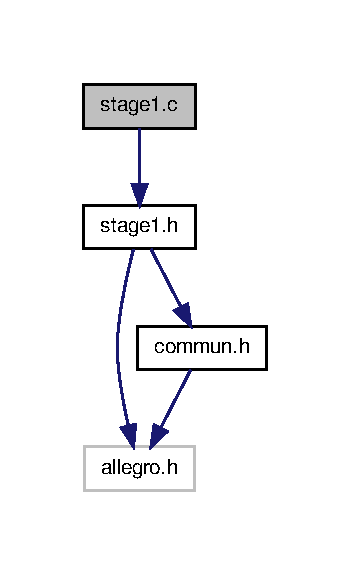
\includegraphics[width=168pt]{stage1_8c__incl}
\end{center}
\end{figure}
\subsection*{Functions}
\begin{DoxyCompactItemize}
\item 
\hypertarget{stage1_8c_a5ea1d3aac92cedac1d41568b0f3d87e2}{void \hyperlink{stage1_8c_a5ea1d3aac92cedac1d41568b0f3d87e2}{init\-\_\-fond11} (\hyperlink{struct_background}{Background} $\ast$fond)}\label{stage1_8c_a5ea1d3aac92cedac1d41568b0f3d87e2}

\begin{DoxyCompactList}\small\item\em cette fonction permet d'initialiser le fond du stage 1 \end{DoxyCompactList}\item 
\hypertarget{stage1_8c_a4268675daa095898f0c55ec1ad9073b6}{void \hyperlink{stage1_8c_a4268675daa095898f0c55ec1ad9073b6}{init\-\_\-frog11} (\hyperlink{struct_froggy}{Froggy} $\ast$frog)}\label{stage1_8c_a4268675daa095898f0c55ec1ad9073b6}

\begin{DoxyCompactList}\small\item\em cette fonction permet d'initialiser \hyperlink{struct_froggy}{Froggy} dans le stage 1 \end{DoxyCompactList}\item 
\hypertarget{stage1_8c_a90a81b35297e49d25db1d71d88606886}{void \hyperlink{stage1_8c_a90a81b35297e49d25db1d71d88606886}{init\-\_\-rat} (\hyperlink{struct_rat}{Rat} $\ast$rat)}\label{stage1_8c_a90a81b35297e49d25db1d71d88606886}

\begin{DoxyCompactList}\small\item\em cette fonction permet d'initialiser le rat dans le stage 1 (img,x,y) \end{DoxyCompactList}\item 
\hypertarget{stage1_8c_a5e72e6ea61d0fd5256da62097b04cb5a}{void \hyperlink{stage1_8c_a5e72e6ea61d0fd5256da62097b04cb5a}{update\-\_\-rat} (\hyperlink{struct_rat}{Rat} $\ast$rat, int step)}\label{stage1_8c_a5e72e6ea61d0fd5256da62097b04cb5a}

\begin{DoxyCompactList}\small\item\em cette fonction permet de mettre à jour la position du \hyperlink{struct_rat}{Rat} au fur et à mesure que la posisition du fond se modifie. On doit faire appel à cette fonction à chaque fois que fond11.\-x augmente ou diminue \end{DoxyCompactList}\item 
int \hyperlink{stage1_8c_a4d5fb26f0e8daa1e2c5f478c43b276d6}{collision\-\_\-rat} (\hyperlink{struct_rat}{Rat} rat, \hyperlink{struct_froggy}{Froggy} frog)
\begin{DoxyCompactList}\small\item\em Cette fonction détecte s'il y a ou non un contact entre le rat et \hyperlink{struct_froggy}{Froggy}. Si celui-\/ci existe elle retourne 1 sinon elle retourne 0. \end{DoxyCompactList}\item 
\hypertarget{stage1_8c_a229f6a88a6aa38754ab45f0c611f1257}{void \hyperlink{stage1_8c_a229f6a88a6aa38754ab45f0c611f1257}{init\-\_\-calque11} (\hyperlink{struct_calque}{Calque} $\ast$calque, \hyperlink{struct_froggy}{Froggy} frog)}\label{stage1_8c_a229f6a88a6aa38754ab45f0c611f1257}

\begin{DoxyCompactList}\small\item\em Cette fonction permet d'initialiser le calque du stage 1 qui est l'image du fond dans lequel les obstacles sont coloriés par des couleurs spécifiques (les trous en blanc de coordonnées 16777215, le plancher en bleu ciel de coordonnées 65535, la zone d'arrivée en orange de coordonnées 16850088) \end{DoxyCompactList}\item 
\hypertarget{stage1_8c_a309d9720fc9954489a3b45f7f8799a07}{int {\bfseries collision\-\_\-blanc11} (\hyperlink{struct_calque}{Calque} calque, int posx\-\_\-blanc, int y)}\label{stage1_8c_a309d9720fc9954489a3b45f7f8799a07}

\item 
\hypertarget{stage1_8c_aa197ae16449bac3ac6ba99a894238c5c}{void \hyperlink{stage1_8c_aa197ae16449bac3ac6ba99a894238c5c}{chute11} (int test, \hyperlink{struct_froggy}{Froggy} $\ast$frog, int direction)}\label{stage1_8c_aa197ae16449bac3ac6ba99a894238c5c}

\begin{DoxyCompactList}\small\item\em lorsque test est égale à 1, toutes les touches seront bloquées et \hyperlink{struct_froggy}{Froggy} sera absorbée vers le bas \end{DoxyCompactList}\item 
\hypertarget{stage1_8c_a08440d1edfb25fe84471e2fcbf011ad7}{int \hyperlink{stage1_8c_a08440d1edfb25fe84471e2fcbf011ad7}{collision\-\_\-bleu11} (\hyperlink{struct_calque}{Calque} calque, int posx\-\_\-bleu, int y)}\label{stage1_8c_a08440d1edfb25fe84471e2fcbf011ad7}

\begin{DoxyCompactList}\small\item\em Cette fonction permet de détecter la nature de la surface au dessous de la grenouille lorsque celle ci saute(plancher, trou ou vide). Elle retourne 1 si c'est un plancher, 2 si c'est un trou et 0 si c'est du vide. \end{DoxyCompactList}\item 
\hypertarget{stage1_8c_a16cdf575cb8347a95c9cf51db6fe278c}{void \hyperlink{stage1_8c_a16cdf575cb8347a95c9cf51db6fe278c}{init\-\_\-coins11} (\hyperlink{struct_coins}{Coins} $\ast$piece)}\label{stage1_8c_a16cdf575cb8347a95c9cf51db6fe278c}

\begin{DoxyCompactList}\small\item\em cette fonction permet d'initialiser les positions des pièces dans le stage 1 \end{DoxyCompactList}\item 
\hypertarget{stage1_8c_a05cc58d63fb34b61b66287f386e26b92}{int \hyperlink{stage1_8c_a05cc58d63fb34b61b66287f386e26b92}{collision\-\_\-piece11} (int x, int y, int $\ast$test, \hyperlink{struct_coins}{Coins} piece, int nbr\-\_\-p)}\label{stage1_8c_a05cc58d63fb34b61b66287f386e26b92}

\begin{DoxyCompactList}\small\item\em Cette fonction permet de tester si \hyperlink{struct_froggy}{Froggy} entre en collision avec une piece (\hyperlink{struct_coins}{Coins}) ou non. test prend 1 si la collision existe et 0 si celle-\/ci n'existe pas. elle retourne la position de la pièce avec laquelle il y a eu collision. \end{DoxyCompactList}\item 
\hypertarget{stage1_8c_a71762fca2faaf2856c86384b15f3448c}{void \hyperlink{stage1_8c_a71762fca2faaf2856c86384b15f3448c}{destroy\-\_\-rat} (\hyperlink{struct_rat}{Rat} $\ast$rat)}\label{stage1_8c_a71762fca2faaf2856c86384b15f3448c}

\begin{DoxyCompactList}\small\item\em Cette fonction permet de libérer la mémoire allouée pour la structure \hyperlink{struct_rat}{Rat}. \end{DoxyCompactList}\item 
\hypertarget{stage1_8c_add8f7f0d91a85230e4272444fe3295e0}{void \hyperlink{stage1_8c_add8f7f0d91a85230e4272444fe3295e0}{aspiration} (int test, \hyperlink{struct_froggy}{Froggy} $\ast$frog, int direction, int $\ast$aspiration\-\_\-terminee)}\label{stage1_8c_add8f7f0d91a85230e4272444fe3295e0}

\begin{DoxyCompactList}\small\item\em lorsque test est égale à 1, toutes les touches seront bloquées et \hyperlink{struct_froggy}{Froggy} sera absorbée vers le haut \end{DoxyCompactList}\item 
\hypertarget{stage1_8c_a790cdeddbf49ce807d36bf5fa853da8d}{void \hyperlink{stage1_8c_a790cdeddbf49ce807d36bf5fa853da8d}{fonction\-\_\-stage1} (int $\ast$stage1\-\_\-termine, int $\ast$direction11, int $\ast$key\-\_\-pressed11, int $\ast$frame\-\_\-counter11, int $\ast$test\-\_\-chute11, int $\ast$saut\-\_\-horizontal11, int $\ast$rat\-\_\-counter, int $\ast$vie11, int $\ast$bloquer\-\_\-collision\-\_\-rat, int $\ast$compteur\-\_\-collision\-\_\-rat, int $\ast$nbr\-\_\-piece11, int $\ast$score11, int $\ast$test\-\_\-aspiration, int $\ast$aspiration\-\_\-terminee, \hyperlink{struct_background}{Background} $\ast$fond11, \hyperlink{struct_froggy}{Froggy} $\ast$frog11, \hyperlink{struct_calque}{Calque} $\ast$calque11, \hyperlink{struct_rat}{Rat} $\ast$rat, \hyperlink{struct_coins}{Coins} $\ast$piece11, \hyperlink{struct_pause}{Pause} pause, B\-I\-T\-M\-A\-P $\ast$Cursor, int $\ast$saut\-\_\-vertical11, int $\ast$top11)}\label{stage1_8c_a790cdeddbf49ce807d36bf5fa853da8d}

\begin{DoxyCompactList}\small\item\em Cette fonction permet de faire appel aux fonctions du stage 1. \end{DoxyCompactList}\end{DoxyCompactItemize}
\subsection*{Variables}
\begin{DoxyCompactItemize}
\item 
B\-I\-T\-M\-A\-P $\ast$ \hyperlink{stage1_8c_a700c2011fa3d781837c4d795a70c7c9d}{Buffer}
\begin{DoxyCompactList}\small\item\em Ceci est la déclaration du Buffer comme étant variable globale. \end{DoxyCompactList}\end{DoxyCompactItemize}


\subsection{Detailed Description}
\begin{DoxyAuthor}{Author}
Las Vegas 
\end{DoxyAuthor}
\begin{DoxyDate}{Date}
22 Mai 2013 
\end{DoxyDate}


\subsection{Function Documentation}
\hypertarget{stage1_8c_a4d5fb26f0e8daa1e2c5f478c43b276d6}{\index{stage1.\-c@{stage1.\-c}!collision\-\_\-rat@{collision\-\_\-rat}}
\index{collision\-\_\-rat@{collision\-\_\-rat}!stage1.c@{stage1.\-c}}
\subsubsection[{collision\-\_\-rat}]{\setlength{\rightskip}{0pt plus 5cm}int collision\-\_\-rat (
\begin{DoxyParamCaption}
\item[{{\bf Rat}}]{rat, }
\item[{{\bf Froggy}}]{frog}
\end{DoxyParamCaption}
)}}\label{stage1_8c_a4d5fb26f0e8daa1e2c5f478c43b276d6}


Cette fonction détecte s'il y a ou non un contact entre le rat et \hyperlink{struct_froggy}{Froggy}. Si celui-\/ci existe elle retourne 1 sinon elle retourne 0. 

Cette fonction permet de détecter la nature de la surface au dessous de la grenouille lorsque celle ci se déplace vers la droite ou vers la gauche(plancher, trou ou vide). Elle retourne 1 si c'est un plancher, 2 si c'est un trou et 0 si c'est du vide. 

Here is the caller graph for this function\-:\nopagebreak
\begin{figure}[H]
\begin{center}
\leavevmode
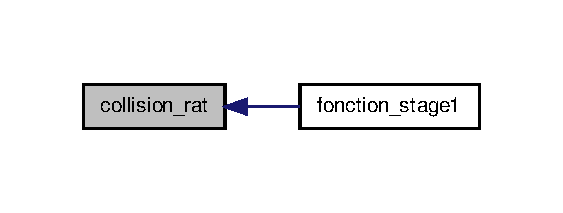
\includegraphics[width=270pt]{stage1_8c_a4d5fb26f0e8daa1e2c5f478c43b276d6_icgraph}
\end{center}
\end{figure}




\subsection{Variable Documentation}
\hypertarget{stage1_8c_a700c2011fa3d781837c4d795a70c7c9d}{\index{stage1.\-c@{stage1.\-c}!Buffer@{Buffer}}
\index{Buffer@{Buffer}!stage1.c@{stage1.\-c}}
\subsubsection[{Buffer}]{\setlength{\rightskip}{0pt plus 5cm}B\-I\-T\-M\-A\-P$\ast$ Buffer}}\label{stage1_8c_a700c2011fa3d781837c4d795a70c7c9d}


Ceci est la déclaration du Buffer comme étant variable globale. 


\begin{DoxyItemize}
\item 
\end{DoxyItemize}
\hypertarget{stage1_8h}{\section{stage1.\-h File Reference}
\label{stage1_8h}\index{stage1.\-h@{stage1.\-h}}
}
{\ttfamily \#include $<$allegro.\-h$>$}\\*
{\ttfamily \#include \char`\"{}commun.\-h\char`\"{}}\\*
Include dependency graph for stage1.\-h\-:\nopagebreak
\begin{figure}[H]
\begin{center}
\leavevmode
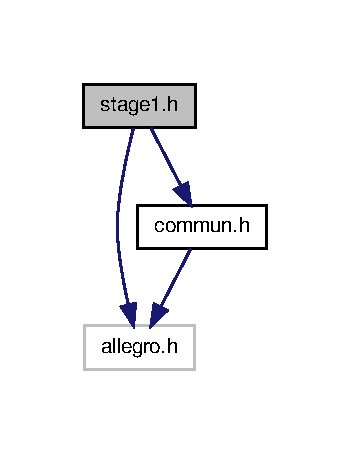
\includegraphics[width=168pt]{stage1_8h__incl}
\end{center}
\end{figure}
This graph shows which files directly or indirectly include this file\-:\nopagebreak
\begin{figure}[H]
\begin{center}
\leavevmode
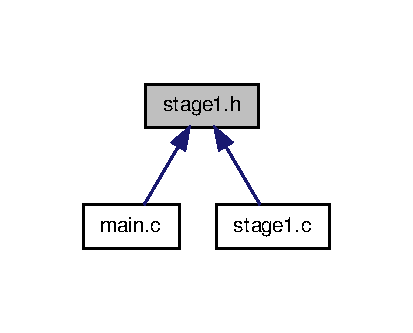
\includegraphics[width=198pt]{stage1_8h__dep__incl}
\end{center}
\end{figure}
\subsection*{Data Structures}
\begin{DoxyCompactItemize}
\item 
struct \hyperlink{struct_rat}{Rat}
\begin{DoxyCompactList}\small\item\em x la position du rat en largeur et y en hauteur. Nous avons 4 voitures dans le jeu donc nous avons besoin de 4 x et de 4 y différents. img est le B\-I\-T\-M\-A\-P de cette voiture puisque elle contient 3 frames donc nous avons 3 images. \end{DoxyCompactList}\end{DoxyCompactItemize}
\subsection*{Macros}
\begin{DoxyCompactItemize}
\item 
\hypertarget{stage1_8h_a2b51498cc7e646f9723907ddbd8440a6}{\#define {\bfseries nbr\-\_\-rat}~4}\label{stage1_8h_a2b51498cc7e646f9723907ddbd8440a6}

\item 
\hypertarget{stage1_8h_aaf3d7b536350d895985aa9b4917adeee}{\#define {\bfseries nbr\-\_\-coins11}~15}\label{stage1_8h_aaf3d7b536350d895985aa9b4917adeee}

\end{DoxyCompactItemize}
\subsection*{Functions}
\begin{DoxyCompactItemize}
\item 
\hypertarget{stage1_8h_a5ea1d3aac92cedac1d41568b0f3d87e2}{void \hyperlink{stage1_8h_a5ea1d3aac92cedac1d41568b0f3d87e2}{init\-\_\-fond11} (\hyperlink{struct_background}{Background} $\ast$fond)}\label{stage1_8h_a5ea1d3aac92cedac1d41568b0f3d87e2}

\begin{DoxyCompactList}\small\item\em cette fonction permet d'initialiser le fond du stage 1 \end{DoxyCompactList}\item 
\hypertarget{stage1_8h_a4268675daa095898f0c55ec1ad9073b6}{void \hyperlink{stage1_8h_a4268675daa095898f0c55ec1ad9073b6}{init\-\_\-frog11} (\hyperlink{struct_froggy}{Froggy} $\ast$frog)}\label{stage1_8h_a4268675daa095898f0c55ec1ad9073b6}

\begin{DoxyCompactList}\small\item\em cette fonction permet d'initialiser \hyperlink{struct_froggy}{Froggy} dans le stage 1 \end{DoxyCompactList}\item 
\hypertarget{stage1_8h_a90a81b35297e49d25db1d71d88606886}{void \hyperlink{stage1_8h_a90a81b35297e49d25db1d71d88606886}{init\-\_\-rat} (\hyperlink{struct_rat}{Rat} $\ast$rat)}\label{stage1_8h_a90a81b35297e49d25db1d71d88606886}

\begin{DoxyCompactList}\small\item\em cette fonction permet d'initialiser le rat dans le stage 1 (img,x,y) \end{DoxyCompactList}\item 
\hypertarget{stage1_8h_a5e72e6ea61d0fd5256da62097b04cb5a}{void \hyperlink{stage1_8h_a5e72e6ea61d0fd5256da62097b04cb5a}{update\-\_\-rat} (\hyperlink{struct_rat}{Rat} $\ast$rat, int step)}\label{stage1_8h_a5e72e6ea61d0fd5256da62097b04cb5a}

\begin{DoxyCompactList}\small\item\em cette fonction permet de mettre à jour la position du \hyperlink{struct_rat}{Rat} au fur et à mesure que la posisition du fond se modifie. On doit faire appel à cette fonction à chaque fois que fond11.\-x augmente ou diminue \end{DoxyCompactList}\item 
int \hyperlink{stage1_8h_a4d5fb26f0e8daa1e2c5f478c43b276d6}{collision\-\_\-rat} (\hyperlink{struct_rat}{Rat} rat, \hyperlink{struct_froggy}{Froggy} frog)
\begin{DoxyCompactList}\small\item\em Cette fonction détecte s'il y a ou non un contact entre le rat et \hyperlink{struct_froggy}{Froggy}. Si celui-\/ci existe elle retourne 1 sinon elle retourne 0. \end{DoxyCompactList}\item 
\hypertarget{stage1_8h_a229f6a88a6aa38754ab45f0c611f1257}{void \hyperlink{stage1_8h_a229f6a88a6aa38754ab45f0c611f1257}{init\-\_\-calque11} (\hyperlink{struct_calque}{Calque} $\ast$calque, \hyperlink{struct_froggy}{Froggy} frog)}\label{stage1_8h_a229f6a88a6aa38754ab45f0c611f1257}

\begin{DoxyCompactList}\small\item\em Cette fonction permet d'initialiser le calque du stage 1 qui est l'image du fond dans lequel les obstacles sont coloriés par des couleurs spécifiques (les trous en blanc de coordonnées 16777215, le plancher en bleu ciel de coordonnées 65535, la zone d'arrivée en orange de coordonnées 16850088) \end{DoxyCompactList}\item 
\hypertarget{stage1_8h_a309d9720fc9954489a3b45f7f8799a07}{int {\bfseries collision\-\_\-blanc11} (\hyperlink{struct_calque}{Calque} calque, int posx\-\_\-blanc, int y)}\label{stage1_8h_a309d9720fc9954489a3b45f7f8799a07}

\item 
\hypertarget{stage1_8h_aa197ae16449bac3ac6ba99a894238c5c}{void \hyperlink{stage1_8h_aa197ae16449bac3ac6ba99a894238c5c}{chute11} (int test, \hyperlink{struct_froggy}{Froggy} $\ast$frog, int direction)}\label{stage1_8h_aa197ae16449bac3ac6ba99a894238c5c}

\begin{DoxyCompactList}\small\item\em lorsque test est égale à 1, toutes les touches seront bloquées et \hyperlink{struct_froggy}{Froggy} sera absorbée vers le bas \end{DoxyCompactList}\item 
\hypertarget{stage1_8h_a08440d1edfb25fe84471e2fcbf011ad7}{int \hyperlink{stage1_8h_a08440d1edfb25fe84471e2fcbf011ad7}{collision\-\_\-bleu11} (\hyperlink{struct_calque}{Calque} calque, int posx\-\_\-bleu, int y)}\label{stage1_8h_a08440d1edfb25fe84471e2fcbf011ad7}

\begin{DoxyCompactList}\small\item\em Cette fonction permet de détecter la nature de la surface au dessous de la grenouille lorsque celle ci saute(plancher, trou ou vide). Elle retourne 1 si c'est un plancher, 2 si c'est un trou et 0 si c'est du vide. \end{DoxyCompactList}\item 
\hypertarget{stage1_8h_a16cdf575cb8347a95c9cf51db6fe278c}{void \hyperlink{stage1_8h_a16cdf575cb8347a95c9cf51db6fe278c}{init\-\_\-coins11} (\hyperlink{struct_coins}{Coins} $\ast$piece)}\label{stage1_8h_a16cdf575cb8347a95c9cf51db6fe278c}

\begin{DoxyCompactList}\small\item\em cette fonction permet d'initialiser les positions des pièces dans le stage 1 \end{DoxyCompactList}\item 
\hypertarget{stage1_8h_a05cc58d63fb34b61b66287f386e26b92}{int \hyperlink{stage1_8h_a05cc58d63fb34b61b66287f386e26b92}{collision\-\_\-piece11} (int x, int y, int $\ast$test, \hyperlink{struct_coins}{Coins} piece, int nbr\-\_\-p)}\label{stage1_8h_a05cc58d63fb34b61b66287f386e26b92}

\begin{DoxyCompactList}\small\item\em Cette fonction permet de tester si \hyperlink{struct_froggy}{Froggy} entre en collision avec une piece (\hyperlink{struct_coins}{Coins}) ou non. test prend 1 si la collision existe et 0 si celle-\/ci n'existe pas. elle retourne la position de la pièce avec laquelle il y a eu collision. \end{DoxyCompactList}\item 
\hypertarget{stage1_8h_a71762fca2faaf2856c86384b15f3448c}{void \hyperlink{stage1_8h_a71762fca2faaf2856c86384b15f3448c}{destroy\-\_\-rat} (\hyperlink{struct_rat}{Rat} $\ast$rat)}\label{stage1_8h_a71762fca2faaf2856c86384b15f3448c}

\begin{DoxyCompactList}\small\item\em Cette fonction permet de libérer la mémoire allouée pour la structure \hyperlink{struct_rat}{Rat}. \end{DoxyCompactList}\item 
\hypertarget{stage1_8h_add8f7f0d91a85230e4272444fe3295e0}{void \hyperlink{stage1_8h_add8f7f0d91a85230e4272444fe3295e0}{aspiration} (int test, \hyperlink{struct_froggy}{Froggy} $\ast$frog, int direction, int $\ast$aspiration\-\_\-terminee)}\label{stage1_8h_add8f7f0d91a85230e4272444fe3295e0}

\begin{DoxyCompactList}\small\item\em lorsque test est égale à 1, toutes les touches seront bloquées et \hyperlink{struct_froggy}{Froggy} sera absorbée vers le haut \end{DoxyCompactList}\item 
\hypertarget{stage1_8h_a790cdeddbf49ce807d36bf5fa853da8d}{void \hyperlink{stage1_8h_a790cdeddbf49ce807d36bf5fa853da8d}{fonction\-\_\-stage1} (int $\ast$stage1\-\_\-termine, int $\ast$direction11, int $\ast$key\-\_\-pressed11, int $\ast$frame\-\_\-counter11, int $\ast$test\-\_\-chute11, int $\ast$saut\-\_\-horizontal11, int $\ast$rat\-\_\-counter, int $\ast$vie11, int $\ast$bloquer\-\_\-collision\-\_\-rat, int $\ast$compteur\-\_\-collision\-\_\-rat, int $\ast$nbr\-\_\-piece11, int $\ast$score11, int $\ast$test\-\_\-aspiration, int $\ast$aspiration\-\_\-terminee, \hyperlink{struct_background}{Background} $\ast$fond11, \hyperlink{struct_froggy}{Froggy} $\ast$frog11, \hyperlink{struct_calque}{Calque} $\ast$calque11, \hyperlink{struct_rat}{Rat} $\ast$rat, \hyperlink{struct_coins}{Coins} $\ast$piece11, \hyperlink{struct_pause}{Pause} pause, B\-I\-T\-M\-A\-P $\ast$Cursor, int $\ast$saut\-\_\-vertical11, int $\ast$top11)}\label{stage1_8h_a790cdeddbf49ce807d36bf5fa853da8d}

\begin{DoxyCompactList}\small\item\em Cette fonction permet de faire appel aux fonctions du stage 1. \end{DoxyCompactList}\end{DoxyCompactItemize}


\subsection{Detailed Description}
\begin{DoxyAuthor}{Author}
Las Vegas 
\end{DoxyAuthor}
\begin{DoxyDate}{Date}
22 Mai 2013 
\end{DoxyDate}


\subsection{Function Documentation}
\hypertarget{stage1_8h_a4d5fb26f0e8daa1e2c5f478c43b276d6}{\index{stage1.\-h@{stage1.\-h}!collision\-\_\-rat@{collision\-\_\-rat}}
\index{collision\-\_\-rat@{collision\-\_\-rat}!stage1.h@{stage1.\-h}}
\subsubsection[{collision\-\_\-rat}]{\setlength{\rightskip}{0pt plus 5cm}int collision\-\_\-rat (
\begin{DoxyParamCaption}
\item[{{\bf Rat}}]{rat, }
\item[{{\bf Froggy}}]{frog}
\end{DoxyParamCaption}
)}}\label{stage1_8h_a4d5fb26f0e8daa1e2c5f478c43b276d6}


Cette fonction détecte s'il y a ou non un contact entre le rat et \hyperlink{struct_froggy}{Froggy}. Si celui-\/ci existe elle retourne 1 sinon elle retourne 0. 

Cette fonction permet de détecter la nature de la surface au dessous de la grenouille lorsque celle ci se déplace vers la droite ou vers la gauche(plancher, trou ou vide). Elle retourne 1 si c'est un plancher, 2 si c'est un trou et 0 si c'est du vide. 

Here is the caller graph for this function\-:\nopagebreak
\begin{figure}[H]
\begin{center}
\leavevmode
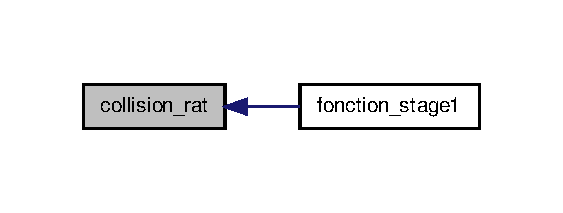
\includegraphics[width=270pt]{stage1_8h_a4d5fb26f0e8daa1e2c5f478c43b276d6_icgraph}
\end{center}
\end{figure}



\hypertarget{stage1__2_8c}{\section{stage1\-\_\-2.\-c File Reference}
\label{stage1__2_8c}\index{stage1\-\_\-2.\-c@{stage1\-\_\-2.\-c}}
}
{\ttfamily \#include \char`\"{}stage1\-\_\-2.\-h\char`\"{}}\\*
Include dependency graph for stage1\-\_\-2.\-c\-:\nopagebreak
\begin{figure}[H]
\begin{center}
\leavevmode
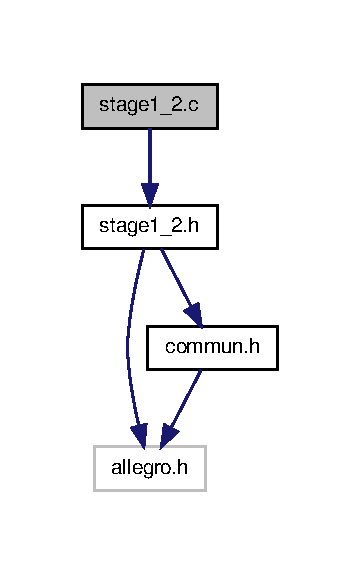
\includegraphics[width=173pt]{stage1__2_8c__incl}
\end{center}
\end{figure}
\subsection*{Functions}
\begin{DoxyCompactItemize}
\item 
\hypertarget{stage1__2_8c_af62f19d4cc21f92f725de7165d7f10ce}{void \hyperlink{stage1__2_8c_af62f19d4cc21f92f725de7165d7f10ce}{init\-\_\-fond12} (\hyperlink{struct_background}{Background} $\ast$fond)}\label{stage1__2_8c_af62f19d4cc21f92f725de7165d7f10ce}

\begin{DoxyCompactList}\small\item\em cette fonction permet d'initialiser le fond du stage 2 \end{DoxyCompactList}\item 
\hypertarget{stage1__2_8c_a0aa521be8b71251bc324c5b174aecd86}{void {\bfseries init\-\_\-frog12} (\hyperlink{struct_froggy}{Froggy} $\ast$frog)}\label{stage1__2_8c_a0aa521be8b71251bc324c5b174aecd86}

\item 
\hypertarget{stage1__2_8c_a7a9a17af92ee7bafe10b482a4fb6b84a}{void {\bfseries init\-\_\-calque12} (\hyperlink{struct_calque}{Calque} $\ast$calque, \hyperlink{struct_froggy}{Froggy} frog)}\label{stage1__2_8c_a7a9a17af92ee7bafe10b482a4fb6b84a}

\item 
\hypertarget{stage1__2_8c_a5e466270bb816a223460a1c0682be2ce}{int {\bfseries collision\-\_\-blanc12} (\hyperlink{struct_calque}{Calque} calque, int posx\-\_\-blanc, int y)}\label{stage1__2_8c_a5e466270bb816a223460a1c0682be2ce}

\item 
\hypertarget{stage1__2_8c_a4cd8e9d56c412a2bed1ea897f84e1c75}{void {\bfseries chute12} (int test, \hyperlink{struct_froggy}{Froggy} $\ast$frog, int direction)}\label{stage1__2_8c_a4cd8e9d56c412a2bed1ea897f84e1c75}

\item 
\hypertarget{stage1__2_8c_aa5e4fd79fa38ccfc1e7b801db680df7c}{int {\bfseries collision\-\_\-bleu12} (\hyperlink{struct_calque}{Calque} calque, int posx\-\_\-bleu, int y)}\label{stage1__2_8c_aa5e4fd79fa38ccfc1e7b801db680df7c}

\item 
\hypertarget{stage1__2_8c_a0e3537bdb62c5d3a97ddd3ae9611fa3b}{void {\bfseries init\-\_\-coins12} (\hyperlink{struct_coins}{Coins} $\ast$piece)}\label{stage1__2_8c_a0e3537bdb62c5d3a97ddd3ae9611fa3b}

\item 
\hypertarget{stage1__2_8c_a6c0e87699e8c385adc83aa2b18eff750}{int {\bfseries collision\-\_\-piece12} (int x, int y, int $\ast$test, \hyperlink{struct_coins}{Coins} piece, int nbr\-\_\-p)}\label{stage1__2_8c_a6c0e87699e8c385adc83aa2b18eff750}

\item 
\hypertarget{stage1__2_8c_ab0bcd59161b5d1756f4ece8fdf450fd4}{void {\bfseries init\-\_\-voiture} (\hyperlink{struct_voiture}{Voiture} $\ast$voiture)}\label{stage1__2_8c_ab0bcd59161b5d1756f4ece8fdf450fd4}

\item 
\hypertarget{stage1__2_8c_a7f7e6e295419e07460efe9099687d4a2}{void {\bfseries update\-\_\-voiture} (\hyperlink{struct_voiture}{Voiture} $\ast$voiture, int step)}\label{stage1__2_8c_a7f7e6e295419e07460efe9099687d4a2}

\item 
\hypertarget{stage1__2_8c_a1b6372ac2a6bb56b51866cde64c780bb}{void {\bfseries destroy\-\_\-voiture} (\hyperlink{struct_voiture}{Voiture} $\ast$voiture)}\label{stage1__2_8c_a1b6372ac2a6bb56b51866cde64c780bb}

\item 
\hypertarget{stage1__2_8c_a929928f7e3ecac9b000168d7fa3bb3fb}{void {\bfseries fonctions\-\_\-stage1\-\_\-2} (int $\ast$direction12, int $\ast$key\-\_\-pressed12, int $\ast$frame\-\_\-counter12, int $\ast$test\-\_\-chute12, int $\ast$saut\-\_\-horizontal12, int $\ast$nbr\-\_\-piece12, int $\ast$score12, int $\ast$saut\-\_\-vertical12, int $\ast$top12, int $\ast$car\-\_\-counter, int $\ast$stage12\-\_\-termine, int $\ast$win\-\_\-stage12, int $\ast$bloquer\-\_\-voiture, \hyperlink{struct_background}{Background} $\ast$fond12, \hyperlink{struct_froggy}{Froggy} $\ast$frog12, \hyperlink{struct_calque}{Calque} $\ast$calque12, \hyperlink{struct_coins}{Coins} $\ast$piece12, \hyperlink{struct_voiture}{Voiture} $\ast$voiture, \hyperlink{struct_pause}{Pause} pause, B\-I\-T\-M\-A\-P $\ast$Cursor)}\label{stage1__2_8c_a929928f7e3ecac9b000168d7fa3bb3fb}

\end{DoxyCompactItemize}
\subsection*{Variables}
\begin{DoxyCompactItemize}
\item 
B\-I\-T\-M\-A\-P $\ast$ \hyperlink{stage1__2_8c_a700c2011fa3d781837c4d795a70c7c9d}{Buffer}
\begin{DoxyCompactList}\small\item\em Ceci est la déclaration du Buffer comme étant variable globale. \end{DoxyCompactList}\end{DoxyCompactItemize}


\subsection{Detailed Description}
\begin{DoxyAuthor}{Author}
Las Vegas 
\end{DoxyAuthor}
\begin{DoxyDate}{Date}
22 Mai 2013 
\end{DoxyDate}


\subsection{Variable Documentation}
\hypertarget{stage1__2_8c_a700c2011fa3d781837c4d795a70c7c9d}{\index{stage1\-\_\-2.\-c@{stage1\-\_\-2.\-c}!Buffer@{Buffer}}
\index{Buffer@{Buffer}!stage1_2.c@{stage1\-\_\-2.\-c}}
\subsubsection[{Buffer}]{\setlength{\rightskip}{0pt plus 5cm}B\-I\-T\-M\-A\-P$\ast$ Buffer}}\label{stage1__2_8c_a700c2011fa3d781837c4d795a70c7c9d}


Ceci est la déclaration du Buffer comme étant variable globale. 


\begin{DoxyItemize}
\item 
\end{DoxyItemize}
\hypertarget{stage1__2_8h}{\section{stage1\-\_\-2.\-h File Reference}
\label{stage1__2_8h}\index{stage1\-\_\-2.\-h@{stage1\-\_\-2.\-h}}
}
{\ttfamily \#include $<$allegro.\-h$>$}\\*
{\ttfamily \#include \char`\"{}commun.\-h\char`\"{}}\\*
Include dependency graph for stage1\-\_\-2.\-h\-:\nopagebreak
\begin{figure}[H]
\begin{center}
\leavevmode
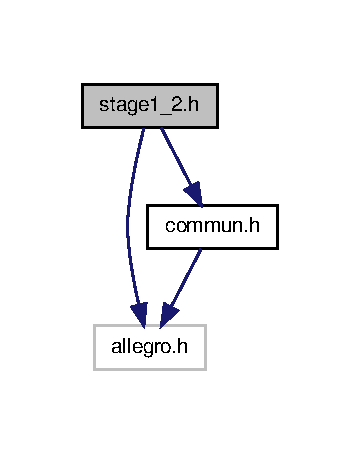
\includegraphics[width=173pt]{stage1__2_8h__incl}
\end{center}
\end{figure}
This graph shows which files directly or indirectly include this file\-:\nopagebreak
\begin{figure}[H]
\begin{center}
\leavevmode
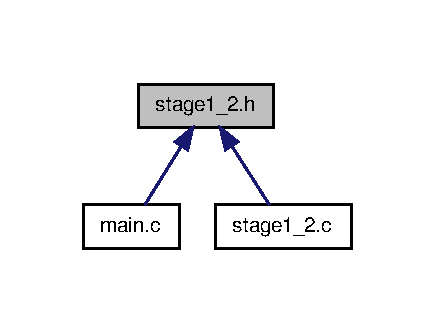
\includegraphics[width=208pt]{stage1__2_8h__dep__incl}
\end{center}
\end{figure}
\subsection*{Data Structures}
\begin{DoxyCompactItemize}
\item 
struct \hyperlink{struct_voiture}{Voiture}
\begin{DoxyCompactList}\small\item\em x la position de la voiture en largeur et y en hauteur. Nous avons 4 voitures dans le jeu donc nous avons besoin de 4 x et de 4 y différents. img est le B\-I\-T\-M\-A\-P de cette voiture puisque elle contient 5 positions donc nous avons 5 images. \end{DoxyCompactList}\end{DoxyCompactItemize}
\subsection*{Macros}
\begin{DoxyCompactItemize}
\item 
\hypertarget{stage1__2_8h_a1505178be35a978e1d77e1dc10a5f3d9}{\#define {\bfseries nbr\-\_\-coins12}~12}\label{stage1__2_8h_a1505178be35a978e1d77e1dc10a5f3d9}

\item 
\hypertarget{stage1__2_8h_a34f5bda2e28e3c127dcbdbfa7f09e350}{\#define {\bfseries nbr\-\_\-voiture}~4}\label{stage1__2_8h_a34f5bda2e28e3c127dcbdbfa7f09e350}

\end{DoxyCompactItemize}
\subsection*{Functions}
\begin{DoxyCompactItemize}
\item 
\hypertarget{stage1__2_8h_af62f19d4cc21f92f725de7165d7f10ce}{void \hyperlink{stage1__2_8h_af62f19d4cc21f92f725de7165d7f10ce}{init\-\_\-fond12} (\hyperlink{struct_background}{Background} $\ast$fond)}\label{stage1__2_8h_af62f19d4cc21f92f725de7165d7f10ce}

\begin{DoxyCompactList}\small\item\em cette fonction permet d'initialiser le fond du stage 2 \end{DoxyCompactList}\item 
\hypertarget{stage1__2_8h_a0aa521be8b71251bc324c5b174aecd86}{void {\bfseries init\-\_\-frog12} (\hyperlink{struct_froggy}{Froggy} $\ast$frog)}\label{stage1__2_8h_a0aa521be8b71251bc324c5b174aecd86}

\item 
\hypertarget{stage1__2_8h_a7a9a17af92ee7bafe10b482a4fb6b84a}{void {\bfseries init\-\_\-calque12} (\hyperlink{struct_calque}{Calque} $\ast$calque, \hyperlink{struct_froggy}{Froggy} frog)}\label{stage1__2_8h_a7a9a17af92ee7bafe10b482a4fb6b84a}

\item 
\hypertarget{stage1__2_8h_a5e466270bb816a223460a1c0682be2ce}{int {\bfseries collision\-\_\-blanc12} (\hyperlink{struct_calque}{Calque} calque, int posx\-\_\-blanc, int y)}\label{stage1__2_8h_a5e466270bb816a223460a1c0682be2ce}

\item 
\hypertarget{stage1__2_8h_a4cd8e9d56c412a2bed1ea897f84e1c75}{void {\bfseries chute12} (int test, \hyperlink{struct_froggy}{Froggy} $\ast$frog, int direction)}\label{stage1__2_8h_a4cd8e9d56c412a2bed1ea897f84e1c75}

\item 
\hypertarget{stage1__2_8h_aa5e4fd79fa38ccfc1e7b801db680df7c}{int {\bfseries collision\-\_\-bleu12} (\hyperlink{struct_calque}{Calque} calque, int posx\-\_\-bleu, int y)}\label{stage1__2_8h_aa5e4fd79fa38ccfc1e7b801db680df7c}

\item 
\hypertarget{stage1__2_8h_a0e3537bdb62c5d3a97ddd3ae9611fa3b}{void {\bfseries init\-\_\-coins12} (\hyperlink{struct_coins}{Coins} $\ast$piece)}\label{stage1__2_8h_a0e3537bdb62c5d3a97ddd3ae9611fa3b}

\item 
\hypertarget{stage1__2_8h_a6c0e87699e8c385adc83aa2b18eff750}{int {\bfseries collision\-\_\-piece12} (int x, int y, int $\ast$test, \hyperlink{struct_coins}{Coins} piece, int nbr\-\_\-p)}\label{stage1__2_8h_a6c0e87699e8c385adc83aa2b18eff750}

\item 
\hypertarget{stage1__2_8h_ab0bcd59161b5d1756f4ece8fdf450fd4}{void {\bfseries init\-\_\-voiture} (\hyperlink{struct_voiture}{Voiture} $\ast$voiture)}\label{stage1__2_8h_ab0bcd59161b5d1756f4ece8fdf450fd4}

\item 
\hypertarget{stage1__2_8h_a7f7e6e295419e07460efe9099687d4a2}{void {\bfseries update\-\_\-voiture} (\hyperlink{struct_voiture}{Voiture} $\ast$voiture, int step)}\label{stage1__2_8h_a7f7e6e295419e07460efe9099687d4a2}

\item 
\hypertarget{stage1__2_8h_a1b6372ac2a6bb56b51866cde64c780bb}{void {\bfseries destroy\-\_\-voiture} (\hyperlink{struct_voiture}{Voiture} $\ast$voiture)}\label{stage1__2_8h_a1b6372ac2a6bb56b51866cde64c780bb}

\item 
\hypertarget{stage1__2_8h_a929928f7e3ecac9b000168d7fa3bb3fb}{void {\bfseries fonctions\-\_\-stage1\-\_\-2} (int $\ast$direction12, int $\ast$key\-\_\-pressed12, int $\ast$frame\-\_\-counter12, int $\ast$test\-\_\-chute12, int $\ast$saut\-\_\-horizontal12, int $\ast$nbr\-\_\-piece12, int $\ast$score12, int $\ast$saut\-\_\-vertical12, int $\ast$top12, int $\ast$car\-\_\-counter, int $\ast$stage12\-\_\-termine, int $\ast$win\-\_\-stage12, int $\ast$bloquer\-\_\-voiture, \hyperlink{struct_background}{Background} $\ast$fond12, \hyperlink{struct_froggy}{Froggy} $\ast$frog12, \hyperlink{struct_calque}{Calque} $\ast$calque12, \hyperlink{struct_coins}{Coins} $\ast$piece12, \hyperlink{struct_voiture}{Voiture} $\ast$voiture, \hyperlink{struct_pause}{Pause} pause, B\-I\-T\-M\-A\-P $\ast$Cursor)}\label{stage1__2_8h_a929928f7e3ecac9b000168d7fa3bb3fb}

\end{DoxyCompactItemize}


\subsection{Detailed Description}
\begin{DoxyAuthor}{Author}
Las Vegas 
\end{DoxyAuthor}
\begin{DoxyDate}{Date}
22 Mai 2013 
\end{DoxyDate}

\hypertarget{stage2_8c}{\section{stage2.\-c File Reference}
\label{stage2_8c}\index{stage2.\-c@{stage2.\-c}}
}
{\ttfamily \#include \char`\"{}stage2.\-h\char`\"{}}\\*
{\ttfamily \#include \char`\"{}commun.\-h\char`\"{}}\\*
Include dependency graph for stage2.\-c\-:\nopagebreak
\begin{figure}[H]
\begin{center}
\leavevmode
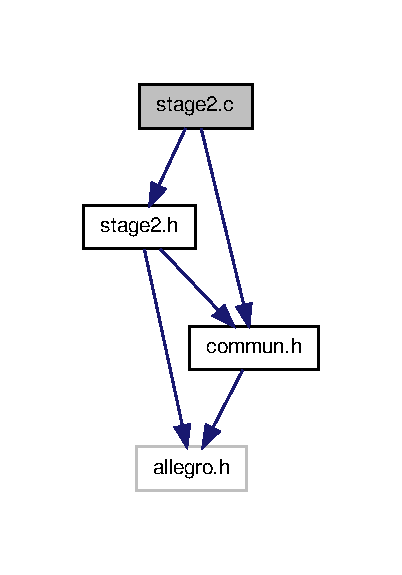
\includegraphics[width=193pt]{stage2_8c__incl}
\end{center}
\end{figure}
\subsection*{Functions}
\begin{DoxyCompactItemize}
\item 
\hypertarget{stage2_8c_a7986de8f5648141ba737c8b3ce6885b7}{void \hyperlink{stage2_8c_a7986de8f5648141ba737c8b3ce6885b7}{init\-\_\-coins2} (\hyperlink{struct_coins}{Coins} $\ast$piece, int xfond)}\label{stage2_8c_a7986de8f5648141ba737c8b3ce6885b7}

\begin{DoxyCompactList}\small\item\em cette fonction permet d'initialiser la position des pièces \end{DoxyCompactList}\item 
\hypertarget{stage2_8c_a516ca48e699498bd5ccba9413c5ecad6}{void \hyperlink{stage2_8c_a516ca48e699498bd5ccba9413c5ecad6}{increment\-\_\-speed\-\_\-counter} ()}\label{stage2_8c_a516ca48e699498bd5ccba9413c5ecad6}

\begin{DoxyCompactList}\small\item\em cette fonction permet d'incrementer le compteur speed\-\_\-counter \end{DoxyCompactList}\item 
\hypertarget{stage2_8c_aac47d9a1e1b7bf8fd0a6169b465ee48b}{{\bfseries E\-N\-D\-\_\-\-O\-F\-\_\-\-F\-U\-N\-C\-T\-I\-O\-N} (\hyperlink{stage2_8h_a516ca48e699498bd5ccba9413c5ecad6}{increment\-\_\-speed\-\_\-counter})}\label{stage2_8c_aac47d9a1e1b7bf8fd0a6169b465ee48b}

\item 
\hypertarget{stage2_8c_a97475d2d7e70aff142a09ca81dd04d4e}{void \hyperlink{stage2_8c_a97475d2d7e70aff142a09ca81dd04d4e}{init\-\_\-speed\-\_\-counter} ()}\label{stage2_8c_a97475d2d7e70aff142a09ca81dd04d4e}

\begin{DoxyCompactList}\small\item\em cette fonction permet d'initialiser le compteur speed\-\_\-counter \end{DoxyCompactList}\item 
\hypertarget{stage2_8c_ae13a70ce6d85919f620581f36b3e2cdd}{void \hyperlink{stage2_8c_ae13a70ce6d85919f620581f36b3e2cdd}{init\-\_\-pigeon} (\hyperlink{struct_pigeon}{Pigeon} $\ast$pigeon)}\label{stage2_8c_ae13a70ce6d85919f620581f36b3e2cdd}

\begin{DoxyCompactList}\small\item\em cette fonction permet d'initialiser la position du \hyperlink{struct_pigeon}{Pigeon} \end{DoxyCompactList}\item 
\hypertarget{stage2_8c_a31b9609566f0e825ae818e9af5b12e98}{void \hyperlink{stage2_8c_a31b9609566f0e825ae818e9af5b12e98}{init\-\_\-background2} (\hyperlink{struct_background}{Background} $\ast$background)}\label{stage2_8c_a31b9609566f0e825ae818e9af5b12e98}

\begin{DoxyCompactList}\small\item\em cette fonction permet d'initialiser le fond du stage3. \end{DoxyCompactList}\item 
\hypertarget{stage2_8c_ac6bde787b60ae13bb350967577a3d6e9}{void \hyperlink{stage2_8c_ac6bde787b60ae13bb350967577a3d6e9}{init\-\_\-calque2} (\hyperlink{struct_calque}{Calque} $\ast$calque, \hyperlink{struct_pigeon}{Pigeon} pigeon)}\label{stage2_8c_ac6bde787b60ae13bb350967577a3d6e9}

\begin{DoxyCompactList}\small\item\em cette fonction permet d'initialiser le calque qui est l'image du fond dans lequel les obstacles sont coloriés par des couleurs spécifiques(les immeubles en blanc de cordonnées 16777215) \end{DoxyCompactList}\item 
\hypertarget{stage2_8c_a32117787652b715cd1c735a23b12db7b}{void \hyperlink{stage2_8c_a32117787652b715cd1c735a23b12db7b}{chute2} (int test, \hyperlink{struct_pigeon}{Pigeon} $\ast$pigeon)}\label{stage2_8c_a32117787652b715cd1c735a23b12db7b}

\begin{DoxyCompactList}\small\item\em lorsque test est égale à 1 toutes les touches sont bloquées et le \hyperlink{struct_pigeon}{Pigeon} sera absorbé vers le bas \end{DoxyCompactList}\item 
\hypertarget{stage2_8c_a352c13a4967a2eabae31c75ba494eec3}{int \hyperlink{stage2_8c_a352c13a4967a2eabae31c75ba494eec3}{collision2} (\hyperlink{struct_calque}{Calque} calque)}\label{stage2_8c_a352c13a4967a2eabae31c75ba494eec3}

\begin{DoxyCompactList}\small\item\em Cette fonction détecte s'il y a ou non un contact entre les immeubles qui sont en blanc sur le \hyperlink{struct_calque}{Calque} et Pigeon.\-si celle ci existe elle retourne 1 sinon elle retourne 0. \end{DoxyCompactList}\item 
\hypertarget{stage2_8c_ad0d606eae4a1f991ff9d6b66ffa124cf}{int \hyperlink{stage2_8c_ad0d606eae4a1f991ff9d6b66ffa124cf}{collision\-\_\-piece2} (int x, int y, int $\ast$test, \hyperlink{struct_coins}{Coins} piece, int nbr\-\_\-p)}\label{stage2_8c_ad0d606eae4a1f991ff9d6b66ffa124cf}

\begin{DoxyCompactList}\small\item\em Cette fonction permet de tester si le \hyperlink{struct_pigeon}{Pigeon} entre en collision avec une piece (\hyperlink{struct_coins}{Coins}) ou non.\-test prend 1 si la collision existe et 0 si celle-\/ci n'existe pas elle retourne la position de la pièce avec laquelle il ya eu collision. \end{DoxyCompactList}\item 
\hypertarget{stage2_8c_aeace1d463f92bbc327e6b0c7e7d41455}{void \hyperlink{stage2_8c_aeace1d463f92bbc327e6b0c7e7d41455}{destroy\-\_\-pigeon} (\hyperlink{struct_pigeon}{Pigeon} $\ast$pigeon)}\label{stage2_8c_aeace1d463f92bbc327e6b0c7e7d41455}

\begin{DoxyCompactList}\small\item\em Cette fonction permet de libérer la mémoire allouer pour la structure \hyperlink{struct_pigeon}{Pigeon}. \end{DoxyCompactList}\item 
\hypertarget{stage2_8c_a034b209449e318bdd43a2007cac42dcc}{void \hyperlink{stage2_8c_a034b209449e318bdd43a2007cac42dcc}{fonction\-\_\-stage2} (\hyperlink{struct_pigeon}{Pigeon} $\ast$pigeon, \hyperlink{struct_background}{Background} $\ast$fond2, \hyperlink{struct_game}{Game} game\-\_\-over, \hyperlink{struct_calque}{Calque} $\ast$calque2, \hyperlink{struct_coins}{Coins} $\ast$piece2, int $\ast$nbr2, int $\ast$test2, int $\ast$frame\-\_\-counter, int $\ast$key\-\_\-pressed2, \hyperlink{struct_pause}{Pause} pause, B\-I\-T\-M\-A\-P $\ast$Cursor, int $\ast$block\-\_\-speed\-\_\-counter, int $\ast$stage2\-\_\-termine, int $\ast$win\-\_\-stage2, int $\ast$score2)}\label{stage2_8c_a034b209449e318bdd43a2007cac42dcc}

\begin{DoxyCompactList}\small\item\em Cette fonction permet de faire appel aux fonctions du stage3. \end{DoxyCompactList}\end{DoxyCompactItemize}
\subsection*{Variables}
\begin{DoxyCompactItemize}
\item 
B\-I\-T\-M\-A\-P $\ast$ \hyperlink{stage2_8c_a700c2011fa3d781837c4d795a70c7c9d}{Buffer}
\begin{DoxyCompactList}\small\item\em Ceci est la déclaration du Buffer comme étant variable globale. \end{DoxyCompactList}\item 
\hypertarget{stage2_8c_a33ea7eb141a698102c0c4e40e329e01b}{volatile long {\bfseries speed\-\_\-counter} = 0}\label{stage2_8c_a33ea7eb141a698102c0c4e40e329e01b}

\end{DoxyCompactItemize}


\subsection{Detailed Description}
\begin{DoxyAuthor}{Author}
Las Vegas 
\end{DoxyAuthor}
\begin{DoxyDate}{Date}
22 Mai 2013 
\end{DoxyDate}


\subsection{Variable Documentation}
\hypertarget{stage2_8c_a700c2011fa3d781837c4d795a70c7c9d}{\index{stage2.\-c@{stage2.\-c}!Buffer@{Buffer}}
\index{Buffer@{Buffer}!stage2.c@{stage2.\-c}}
\subsubsection[{Buffer}]{\setlength{\rightskip}{0pt plus 5cm}B\-I\-T\-M\-A\-P$\ast$ Buffer}}\label{stage2_8c_a700c2011fa3d781837c4d795a70c7c9d}


Ceci est la déclaration du Buffer comme étant variable globale. 


\begin{DoxyItemize}
\item 
\end{DoxyItemize}
\hypertarget{stage2_8h}{\section{stage2.\-h File Reference}
\label{stage2_8h}\index{stage2.\-h@{stage2.\-h}}
}
{\ttfamily \#include $<$allegro.\-h$>$}\\*
{\ttfamily \#include \char`\"{}commun.\-h\char`\"{}}\\*
Include dependency graph for stage2.\-h\-:\nopagebreak
\begin{figure}[H]
\begin{center}
\leavevmode
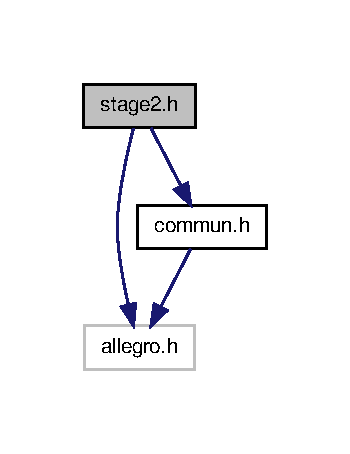
\includegraphics[width=168pt]{stage2_8h__incl}
\end{center}
\end{figure}
This graph shows which files directly or indirectly include this file\-:
\nopagebreak
\begin{figure}[H]
\begin{center}
\leavevmode
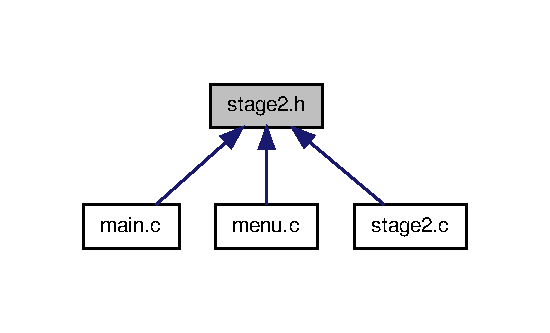
\includegraphics[width=264pt]{stage2_8h__dep__incl}
\end{center}
\end{figure}
\subsection*{Data Structures}
\begin{DoxyCompactItemize}
\item 
struct \hyperlink{struct_pigeon}{Pigeon}
\begin{DoxyCompactList}\small\item\em x la position du \hyperlink{struct_pigeon}{Pigeon} en largeur et y en hauteur. Nous avons un \hyperlink{struct_pigeon}{Pigeon} dans le jeu. img est le B\-I\-T\-M\-A\-P de ce \hyperlink{struct_pigeon}{Pigeon} puisque il contient 5 frames donc nous avons 5 images. \end{DoxyCompactList}\end{DoxyCompactItemize}
\subsection*{Functions}
\begin{DoxyCompactItemize}
\item 
\hypertarget{stage2_8h_a7986de8f5648141ba737c8b3ce6885b7}{void \hyperlink{stage2_8h_a7986de8f5648141ba737c8b3ce6885b7}{init\-\_\-coins2} (\hyperlink{struct_coins}{Coins} $\ast$piece, int xfond)}\label{stage2_8h_a7986de8f5648141ba737c8b3ce6885b7}

\begin{DoxyCompactList}\small\item\em cette fonction permet d'initialiser la position des pièces \end{DoxyCompactList}\item 
\hypertarget{stage2_8h_a516ca48e699498bd5ccba9413c5ecad6}{void \hyperlink{stage2_8h_a516ca48e699498bd5ccba9413c5ecad6}{increment\-\_\-speed\-\_\-counter} ()}\label{stage2_8h_a516ca48e699498bd5ccba9413c5ecad6}

\begin{DoxyCompactList}\small\item\em cette fonction permet d'incrementer le compteur speed\-\_\-counter \end{DoxyCompactList}\item 
\hypertarget{stage2_8h_a97475d2d7e70aff142a09ca81dd04d4e}{void \hyperlink{stage2_8h_a97475d2d7e70aff142a09ca81dd04d4e}{init\-\_\-speed\-\_\-counter} ()}\label{stage2_8h_a97475d2d7e70aff142a09ca81dd04d4e}

\begin{DoxyCompactList}\small\item\em cette fonction permet d'initialiser le compteur speed\-\_\-counter \end{DoxyCompactList}\item 
\hypertarget{stage2_8h_ae13a70ce6d85919f620581f36b3e2cdd}{void \hyperlink{stage2_8h_ae13a70ce6d85919f620581f36b3e2cdd}{init\-\_\-pigeon} (\hyperlink{struct_pigeon}{Pigeon} $\ast$pigeon)}\label{stage2_8h_ae13a70ce6d85919f620581f36b3e2cdd}

\begin{DoxyCompactList}\small\item\em cette fonction permet d'initialiser la position du \hyperlink{struct_pigeon}{Pigeon} \end{DoxyCompactList}\item 
\hypertarget{stage2_8h_a31b9609566f0e825ae818e9af5b12e98}{void \hyperlink{stage2_8h_a31b9609566f0e825ae818e9af5b12e98}{init\-\_\-background2} (\hyperlink{struct_background}{Background} $\ast$background)}\label{stage2_8h_a31b9609566f0e825ae818e9af5b12e98}

\begin{DoxyCompactList}\small\item\em cette fonction permet d'initialiser le fond du stage3. \end{DoxyCompactList}\item 
\hypertarget{stage2_8h_ac6bde787b60ae13bb350967577a3d6e9}{void \hyperlink{stage2_8h_ac6bde787b60ae13bb350967577a3d6e9}{init\-\_\-calque2} (\hyperlink{struct_calque}{Calque} $\ast$calque, \hyperlink{struct_pigeon}{Pigeon} pigeon)}\label{stage2_8h_ac6bde787b60ae13bb350967577a3d6e9}

\begin{DoxyCompactList}\small\item\em cette fonction permet d'initialiser le calque qui est l'image du fond dans lequel les obstacles sont coloriés par des couleurs spécifiques(les immeubles en blanc de cordonnées 16777215) \end{DoxyCompactList}\item 
\hypertarget{stage2_8h_a32117787652b715cd1c735a23b12db7b}{void \hyperlink{stage2_8h_a32117787652b715cd1c735a23b12db7b}{chute2} (int test, \hyperlink{struct_pigeon}{Pigeon} $\ast$pigeon)}\label{stage2_8h_a32117787652b715cd1c735a23b12db7b}

\begin{DoxyCompactList}\small\item\em lorsque test est égale à 1 toutes les touches sont bloquées et le \hyperlink{struct_pigeon}{Pigeon} sera absorbé vers le bas \end{DoxyCompactList}\item 
\hypertarget{stage2_8h_a352c13a4967a2eabae31c75ba494eec3}{int \hyperlink{stage2_8h_a352c13a4967a2eabae31c75ba494eec3}{collision2} (\hyperlink{struct_calque}{Calque} calque)}\label{stage2_8h_a352c13a4967a2eabae31c75ba494eec3}

\begin{DoxyCompactList}\small\item\em Cette fonction détecte s'il y a ou non un contact entre les immeubles qui sont en blanc sur le \hyperlink{struct_calque}{Calque} et Pigeon.\-si celle ci existe elle retourne 1 sinon elle retourne 0. \end{DoxyCompactList}\item 
\hypertarget{stage2_8h_ad0d606eae4a1f991ff9d6b66ffa124cf}{int \hyperlink{stage2_8h_ad0d606eae4a1f991ff9d6b66ffa124cf}{collision\-\_\-piece2} (int x, int y, int $\ast$test, \hyperlink{struct_coins}{Coins} piece, int nbr\-\_\-p)}\label{stage2_8h_ad0d606eae4a1f991ff9d6b66ffa124cf}

\begin{DoxyCompactList}\small\item\em Cette fonction permet de tester si le \hyperlink{struct_pigeon}{Pigeon} entre en collision avec une piece (\hyperlink{struct_coins}{Coins}) ou non.\-test prend 1 si la collision existe et 0 si celle-\/ci n'existe pas elle retourne la position de la pièce avec laquelle il ya eu collision. \end{DoxyCompactList}\item 
\hypertarget{stage2_8h_aeace1d463f92bbc327e6b0c7e7d41455}{void \hyperlink{stage2_8h_aeace1d463f92bbc327e6b0c7e7d41455}{destroy\-\_\-pigeon} (\hyperlink{struct_pigeon}{Pigeon} $\ast$pigeon)}\label{stage2_8h_aeace1d463f92bbc327e6b0c7e7d41455}

\begin{DoxyCompactList}\small\item\em Cette fonction permet de libérer la mémoire allouer pour la structure \hyperlink{struct_pigeon}{Pigeon}. \end{DoxyCompactList}\item 
\hypertarget{stage2_8h_a034b209449e318bdd43a2007cac42dcc}{void \hyperlink{stage2_8h_a034b209449e318bdd43a2007cac42dcc}{fonction\-\_\-stage2} (\hyperlink{struct_pigeon}{Pigeon} $\ast$pigeon, \hyperlink{struct_background}{Background} $\ast$fond2, \hyperlink{struct_game}{Game} game\-\_\-over, \hyperlink{struct_calque}{Calque} $\ast$calque2, \hyperlink{struct_coins}{Coins} $\ast$piece2, int $\ast$nbr2, int $\ast$test2, int $\ast$frame\-\_\-counter, int $\ast$key\-\_\-pressed2, \hyperlink{struct_pause}{Pause} pause, B\-I\-T\-M\-A\-P $\ast$Cursor, int $\ast$block\-\_\-speed\-\_\-counter, int $\ast$stage2\-\_\-termine, int $\ast$win\-\_\-stage2, int $\ast$score2)}\label{stage2_8h_a034b209449e318bdd43a2007cac42dcc}

\begin{DoxyCompactList}\small\item\em Cette fonction permet de faire appel aux fonctions du stage3. \end{DoxyCompactList}\end{DoxyCompactItemize}


\subsection{Detailed Description}
\begin{DoxyAuthor}{Author}
Las Vegas 
\end{DoxyAuthor}
\begin{DoxyDate}{Date}
22 Mai 2013 
\end{DoxyDate}

\hypertarget{stage4_8c}{\section{stage4.\-c File Reference}
\label{stage4_8c}\index{stage4.\-c@{stage4.\-c}}
}
{\ttfamily \#include \char`\"{}stage4.\-h\char`\"{}}\\*
{\ttfamily \#include \char`\"{}commun.\-h\char`\"{}}\\*
Include dependency graph for stage4.\-c\-:\nopagebreak
\begin{figure}[H]
\begin{center}
\leavevmode
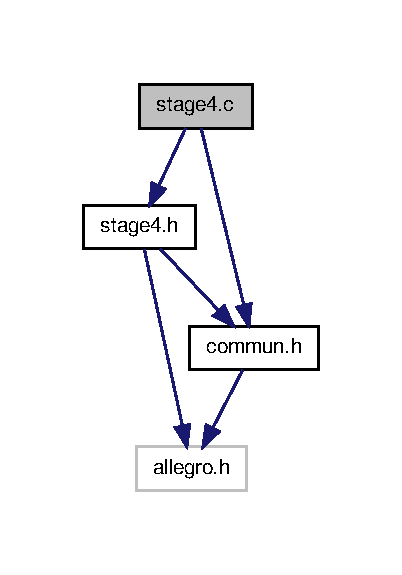
\includegraphics[width=193pt]{stage4_8c__incl}
\end{center}
\end{figure}
\subsection*{Functions}
\begin{DoxyCompactItemize}
\item 
\hypertarget{stage4_8c_a3e9f445b0494a3490683f14e6b46dfe5}{void \hyperlink{stage4_8c_a3e9f445b0494a3490683f14e6b46dfe5}{init\-\_\-frog} (\hyperlink{struct_froggy}{Froggy} $\ast$frog)}\label{stage4_8c_a3e9f445b0494a3490683f14e6b46dfe5}

\begin{DoxyCompactList}\small\item\em cette fonction permet d'initialiser la position du froggy \end{DoxyCompactList}\item 
\hypertarget{stage4_8c_a75d9123eb17a657b2834790e197dcac5}{void \hyperlink{stage4_8c_a75d9123eb17a657b2834790e197dcac5}{init\-\_\-background} (\hyperlink{struct_background}{Background} $\ast$fond)}\label{stage4_8c_a75d9123eb17a657b2834790e197dcac5}

\begin{DoxyCompactList}\small\item\em cette fonction permet d'initialiser le fond du stage 4 \end{DoxyCompactList}\item 
\hypertarget{stage4_8c_a17d7acdb0990f5a795b879b7d4c2a933}{void \hyperlink{stage4_8c_a17d7acdb0990f5a795b879b7d4c2a933}{init\-\_\-calque} (\hyperlink{struct_calque}{Calque} $\ast$calque, \hyperlink{struct_froggy}{Froggy} frog)}\label{stage4_8c_a17d7acdb0990f5a795b879b7d4c2a933}

\begin{DoxyCompactList}\small\item\em cette fonction permet d'initialiser le calque qui est l'image du fond dont le quel les obstacles sont coloriés par des couleurs spécifiques(les trous en blanc de cordonnées 16777215, le plancher en bleu-\/ciel de cordonnées 65535, la zone d'arrivée en orange de cordonnées 16750088) \end{DoxyCompactList}\item 
\hypertarget{stage4_8c_a1741bc4a9095db865859796cdb895397}{int {\bfseries collision\-\_\-blanc} (\hyperlink{struct_calque}{Calque} calque, int posx\-\_\-blanc, int y)}\label{stage4_8c_a1741bc4a9095db865859796cdb895397}

\item 
\hypertarget{stage4_8c_a81f0404b67f1251da4f8241280e64469}{int {\bfseries collision\-\_\-bleu} (\hyperlink{struct_calque}{Calque} calque, int posx\-\_\-bleu, int y)}\label{stage4_8c_a81f0404b67f1251da4f8241280e64469}

\item 
\hypertarget{stage4_8c_a69323fa6a56c0cb78d4aab2505f4afe6}{void \hyperlink{stage4_8c_a69323fa6a56c0cb78d4aab2505f4afe6}{chute} (int test, \hyperlink{struct_froggy}{Froggy} $\ast$frog, int direction)}\label{stage4_8c_a69323fa6a56c0cb78d4aab2505f4afe6}

\begin{DoxyCompactList}\small\item\em Lorsque test est égale 1 toutes les touches sont bloquées et la grenouille sera apsorbé vers le bas. \end{DoxyCompactList}\item 
\hypertarget{stage4_8c_aa6bdce33468efec5b8e309e7bda88fd0}{void \hyperlink{stage4_8c_aa6bdce33468efec5b8e309e7bda88fd0}{init\-\_\-coins} (\hyperlink{struct_coins}{Coins} $\ast$piece, int xfond)}\label{stage4_8c_aa6bdce33468efec5b8e309e7bda88fd0}

\begin{DoxyCompactList}\small\item\em Cette fonction permet d'initialiser les piéces selon x et y. \end{DoxyCompactList}\item 
\hypertarget{stage4_8c_af0679c76661b84549e21c7749ecb51fe}{int {\bfseries collision\-\_\-piece} (int x, int y, int $\ast$test, \hyperlink{struct_coins}{Coins} piece, int nbr\-\_\-p)}\label{stage4_8c_af0679c76661b84549e21c7749ecb51fe}

\item 
\hypertarget{stage4_8c_a3e5b9966f70bb07e205c255bd29675b9}{void \hyperlink{stage4_8c_a3e5b9966f70bb07e205c255bd29675b9}{init\-\_\-serpent} (\hyperlink{struct_serpent}{Serpent} $\ast$serpent)}\label{stage4_8c_a3e5b9966f70bb07e205c255bd29675b9}

\begin{DoxyCompactList}\small\item\em Cette fonction permet d'initialiser le serpent dans le stage4. \end{DoxyCompactList}\item 
\hypertarget{stage4_8c_afcdd9c76d845ada8a020279f178ce7d3}{void \hyperlink{stage4_8c_afcdd9c76d845ada8a020279f178ce7d3}{update\-\_\-serpent} (\hyperlink{struct_serpent}{Serpent} $\ast$serpent, int step)}\label{stage4_8c_afcdd9c76d845ada8a020279f178ce7d3}

\begin{DoxyCompactList}\small\item\em Cette fonction permet de mettre à jour la position du \hyperlink{struct_serpent}{Serpent} au fur et à mesure que la position du fond est modifiée.\-On doit faire appel à cette fonction lorsque font.\-x augmente ou dimminue. \end{DoxyCompactList}\item 
\hypertarget{stage4_8c_a00e6dfd3d7cf49bc6817f445d868105d}{void \hyperlink{stage4_8c_a00e6dfd3d7cf49bc6817f445d868105d}{destroy\-\_\-serpent} (\hyperlink{struct_serpent}{Serpent} $\ast$serpent)}\label{stage4_8c_a00e6dfd3d7cf49bc6817f445d868105d}

\begin{DoxyCompactList}\small\item\em Cette fonction permet de libérer la mémoire allouée pour la structure \hyperlink{struct_serpent}{Serpent}. \end{DoxyCompactList}\item 
\hypertarget{stage4_8c_a45d4d3c05ad3ebd1fc9411b313a49731}{void \hyperlink{stage4_8c_a45d4d3c05ad3ebd1fc9411b313a49731}{init\-\_\-reine} (\hyperlink{struct_reine}{Reine} $\ast$reine)}\label{stage4_8c_a45d4d3c05ad3ebd1fc9411b313a49731}

\begin{DoxyCompactList}\small\item\em Cette fonction permet d'initialiser la reine selon x et y. \end{DoxyCompactList}\item 
\hypertarget{stage4_8c_aa0a8b49219c53b009bcfce9baa6552d9}{void \hyperlink{stage4_8c_aa0a8b49219c53b009bcfce9baa6552d9}{update\-\_\-reine} (\hyperlink{struct_reine}{Reine} $\ast$reine, int step)}\label{stage4_8c_aa0a8b49219c53b009bcfce9baa6552d9}

\begin{DoxyCompactList}\small\item\em Cette fonction permet de mettre à jour la position de la \hyperlink{struct_reine}{Reine} au fur et à mesure que la position du fond est modifiée.\-On doit faire appel à cette fonction lorsque font.\-x augmente ou dimminue. \end{DoxyCompactList}\item 
\hypertarget{stage4_8c_af9c1a3a167f77e034ec20c9a6faa4a22}{int {\bfseries collision\-\_\-serpent} (\hyperlink{struct_serpent}{Serpent} serpent, \hyperlink{struct_froggy}{Froggy} frog)}\label{stage4_8c_af9c1a3a167f77e034ec20c9a6faa4a22}

\item 
\hypertarget{stage4_8c_a688d5f67ac53ba5b4ce809a9b0179749}{int {\bfseries collision\-\_\-reine} (\hyperlink{struct_reine}{Reine} reine, \hyperlink{struct_froggy}{Froggy} frog)}\label{stage4_8c_a688d5f67ac53ba5b4ce809a9b0179749}

\item 
\hypertarget{stage4_8c_a49c10783a23a6940c6a4e02bf48f632d}{void \hyperlink{stage4_8c_a49c10783a23a6940c6a4e02bf48f632d}{destroy\-\_\-reine} (\hyperlink{struct_reine}{Reine} $\ast$reine)}\label{stage4_8c_a49c10783a23a6940c6a4e02bf48f632d}

\begin{DoxyCompactList}\small\item\em Cette fonction permet de libérer la mémoire allouée pour la structure \hyperlink{struct_reine}{Reine}. \end{DoxyCompactList}\item 
\hypertarget{stage4_8c_a879d2cc861461da8a3e06d4ae4e1dc67}{void \hyperlink{stage4_8c_a879d2cc861461da8a3e06d4ae4e1dc67}{fonction\-\_\-stage4} (int $\ast$direction, int $\ast$key\-\_\-pressed, int $\ast$frame\-\_\-counter, int $\ast$serpent\-\_\-counter, int $\ast$reine\-\_\-counter, int $\ast$saut\-\_\-horizontal, int $\ast$test\-\_\-chute, int $\ast$top, int $\ast$saut\-\_\-vertical, int $\ast$nbr\-\_\-p, int $\ast$score4, int $\ast$vie4, int $\ast$compteur\-\_\-collision\-\_\-reine, int $\ast$bloquer\-\_\-collision\-\_\-reine, \hyperlink{struct_background}{Background} $\ast$fond, \hyperlink{struct_froggy}{Froggy} $\ast$frog, \hyperlink{struct_calque}{Calque} $\ast$calque, \hyperlink{struct_coins}{Coins} $\ast$piece, \hyperlink{struct_serpent}{Serpent} $\ast$serpent, \hyperlink{struct_reine}{Reine} $\ast$reine, \hyperlink{struct_pause}{Pause} pause, B\-I\-T\-M\-A\-P $\ast$Cursor, int $\ast$stage\-\_\-termine, int $\ast$win\-\_\-stage, int $\ast$bloquer\-\_\-animation)}\label{stage4_8c_a879d2cc861461da8a3e06d4ae4e1dc67}

\begin{DoxyCompactList}\small\item\em Cette fonction permet de faire l'appel aux fonctions du stage4. \end{DoxyCompactList}\end{DoxyCompactItemize}
\subsection*{Variables}
\begin{DoxyCompactItemize}
\item 
B\-I\-T\-M\-A\-P $\ast$ \hyperlink{stage4_8c_a700c2011fa3d781837c4d795a70c7c9d}{Buffer}
\begin{DoxyCompactList}\small\item\em Ceci est la déclaration du Buffer comme étant variable globale. \end{DoxyCompactList}\end{DoxyCompactItemize}


\subsection{Detailed Description}
\begin{DoxyAuthor}{Author}
Las Vegas 
\end{DoxyAuthor}
\begin{DoxyDate}{Date}
22 Mai 2013 
\end{DoxyDate}


\subsection{Variable Documentation}
\hypertarget{stage4_8c_a700c2011fa3d781837c4d795a70c7c9d}{\index{stage4.\-c@{stage4.\-c}!Buffer@{Buffer}}
\index{Buffer@{Buffer}!stage4.c@{stage4.\-c}}
\subsubsection[{Buffer}]{\setlength{\rightskip}{0pt plus 5cm}B\-I\-T\-M\-A\-P$\ast$ Buffer}}\label{stage4_8c_a700c2011fa3d781837c4d795a70c7c9d}


Ceci est la déclaration du Buffer comme étant variable globale. 


\begin{DoxyItemize}
\item 
\end{DoxyItemize}
\hypertarget{stage4_8h}{\section{stage4.\-h File Reference}
\label{stage4_8h}\index{stage4.\-h@{stage4.\-h}}
}
{\ttfamily \#include $<$allegro.\-h$>$}\\*
{\ttfamily \#include \char`\"{}commun.\-h\char`\"{}}\\*
Include dependency graph for stage4.\-h\-:\nopagebreak
\begin{figure}[H]
\begin{center}
\leavevmode
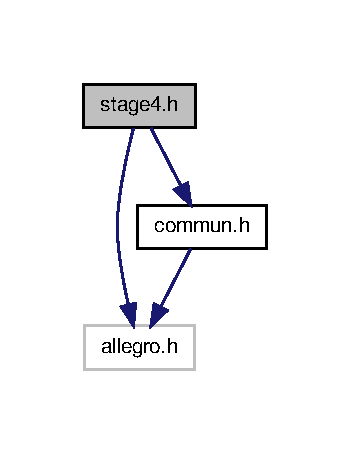
\includegraphics[width=168pt]{stage4_8h__incl}
\end{center}
\end{figure}
This graph shows which files directly or indirectly include this file\-:\nopagebreak
\begin{figure}[H]
\begin{center}
\leavevmode
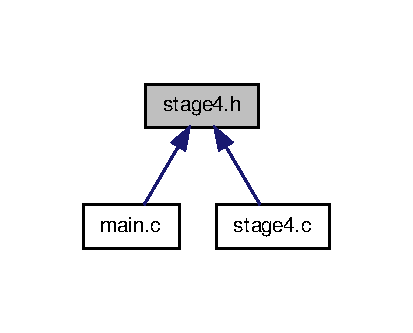
\includegraphics[width=198pt]{stage4_8h__dep__incl}
\end{center}
\end{figure}
\subsection*{Data Structures}
\begin{DoxyCompactItemize}
\item 
struct \hyperlink{struct_serpent}{Serpent}
\begin{DoxyCompactList}\small\item\em x la position du serpent en largeur et y en hauteur. Nous avons 3 serpents dans le jeu donc nous avons besoin de 3 x et de 3 y différents. img est le B\-I\-T\-M\-A\-P de ce serpent puisque il contient 5 positions donc nous avons 5 images. \end{DoxyCompactList}\item 
struct \hyperlink{struct_reine}{Reine}
\begin{DoxyCompactList}\small\item\em x la position de reine en largeur et y en hauteur. Nous avons 3 reines dans le jeu donc nous avons besoin de 3 x et de 3 y différents. img est le B\-I\-T\-M\-A\-P de cette voiture puisque elle contient 5 positions donc nous avons 5 images. \end{DoxyCompactList}\end{DoxyCompactItemize}
\subsection*{Functions}
\begin{DoxyCompactItemize}
\item 
\hypertarget{stage4_8h_a3e9f445b0494a3490683f14e6b46dfe5}{void \hyperlink{stage4_8h_a3e9f445b0494a3490683f14e6b46dfe5}{init\-\_\-frog} (\hyperlink{struct_froggy}{Froggy} $\ast$frog)}\label{stage4_8h_a3e9f445b0494a3490683f14e6b46dfe5}

\begin{DoxyCompactList}\small\item\em cette fonction permet d'initialiser la position du froggy \end{DoxyCompactList}\item 
\hypertarget{stage4_8h_a75d9123eb17a657b2834790e197dcac5}{void \hyperlink{stage4_8h_a75d9123eb17a657b2834790e197dcac5}{init\-\_\-background} (\hyperlink{struct_background}{Background} $\ast$fond)}\label{stage4_8h_a75d9123eb17a657b2834790e197dcac5}

\begin{DoxyCompactList}\small\item\em cette fonction permet d'initialiser le fond du stage 4 \end{DoxyCompactList}\item 
\hypertarget{stage4_8h_a17d7acdb0990f5a795b879b7d4c2a933}{void \hyperlink{stage4_8h_a17d7acdb0990f5a795b879b7d4c2a933}{init\-\_\-calque} (\hyperlink{struct_calque}{Calque} $\ast$calque, \hyperlink{struct_froggy}{Froggy} frog)}\label{stage4_8h_a17d7acdb0990f5a795b879b7d4c2a933}

\begin{DoxyCompactList}\small\item\em cette fonction permet d'initialiser le calque qui est l'image du fond dont le quel les obstacles sont coloriés par des couleurs spécifiques(les trous en blanc de cordonnées 16777215, le plancher en bleu-\/ciel de cordonnées 65535, la zone d'arrivée en orange de cordonnées 16750088) \end{DoxyCompactList}\item 
\hypertarget{stage4_8h_a1741bc4a9095db865859796cdb895397}{int {\bfseries collision\-\_\-blanc} (\hyperlink{struct_calque}{Calque} calque, int posx\-\_\-blanc, int y)}\label{stage4_8h_a1741bc4a9095db865859796cdb895397}

\item 
\hypertarget{stage4_8h_a81f0404b67f1251da4f8241280e64469}{int {\bfseries collision\-\_\-bleu} (\hyperlink{struct_calque}{Calque} calque, int posx\-\_\-bleu, int y)}\label{stage4_8h_a81f0404b67f1251da4f8241280e64469}

\item 
\hypertarget{stage4_8h_a69323fa6a56c0cb78d4aab2505f4afe6}{void \hyperlink{stage4_8h_a69323fa6a56c0cb78d4aab2505f4afe6}{chute} (int test, \hyperlink{struct_froggy}{Froggy} $\ast$frog, int direction)}\label{stage4_8h_a69323fa6a56c0cb78d4aab2505f4afe6}

\begin{DoxyCompactList}\small\item\em Lorsque test est égale 1 toutes les touches sont bloquées et la grenouille sera apsorbé vers le bas. \end{DoxyCompactList}\item 
\hypertarget{stage4_8h_aa6bdce33468efec5b8e309e7bda88fd0}{void \hyperlink{stage4_8h_aa6bdce33468efec5b8e309e7bda88fd0}{init\-\_\-coins} (\hyperlink{struct_coins}{Coins} $\ast$piece, int xfond)}\label{stage4_8h_aa6bdce33468efec5b8e309e7bda88fd0}

\begin{DoxyCompactList}\small\item\em Cette fonction permet d'initialiser les piéces selon x et y. \end{DoxyCompactList}\item 
\hypertarget{stage4_8h_a3e5b9966f70bb07e205c255bd29675b9}{void \hyperlink{stage4_8h_a3e5b9966f70bb07e205c255bd29675b9}{init\-\_\-serpent} (\hyperlink{struct_serpent}{Serpent} $\ast$serpent)}\label{stage4_8h_a3e5b9966f70bb07e205c255bd29675b9}

\begin{DoxyCompactList}\small\item\em Cette fonction permet d'initialiser le serpent dans le stage4. \end{DoxyCompactList}\item 
\hypertarget{stage4_8h_afcdd9c76d845ada8a020279f178ce7d3}{void \hyperlink{stage4_8h_afcdd9c76d845ada8a020279f178ce7d3}{update\-\_\-serpent} (\hyperlink{struct_serpent}{Serpent} $\ast$serpent, int step)}\label{stage4_8h_afcdd9c76d845ada8a020279f178ce7d3}

\begin{DoxyCompactList}\small\item\em Cette fonction permet de mettre à jour la position du \hyperlink{struct_serpent}{Serpent} au fur et à mesure que la position du fond est modifiée.\-On doit faire appel à cette fonction lorsque font.\-x augmente ou dimminue. \end{DoxyCompactList}\item 
\hypertarget{stage4_8h_a00e6dfd3d7cf49bc6817f445d868105d}{void \hyperlink{stage4_8h_a00e6dfd3d7cf49bc6817f445d868105d}{destroy\-\_\-serpent} (\hyperlink{struct_serpent}{Serpent} $\ast$serpent)}\label{stage4_8h_a00e6dfd3d7cf49bc6817f445d868105d}

\begin{DoxyCompactList}\small\item\em Cette fonction permet de libérer la mémoire allouée pour la structure \hyperlink{struct_serpent}{Serpent}. \end{DoxyCompactList}\item 
\hypertarget{stage4_8h_a45d4d3c05ad3ebd1fc9411b313a49731}{void \hyperlink{stage4_8h_a45d4d3c05ad3ebd1fc9411b313a49731}{init\-\_\-reine} (\hyperlink{struct_reine}{Reine} $\ast$reine)}\label{stage4_8h_a45d4d3c05ad3ebd1fc9411b313a49731}

\begin{DoxyCompactList}\small\item\em Cette fonction permet d'initialiser la reine selon x et y. \end{DoxyCompactList}\item 
\hypertarget{stage4_8h_aa0a8b49219c53b009bcfce9baa6552d9}{void \hyperlink{stage4_8h_aa0a8b49219c53b009bcfce9baa6552d9}{update\-\_\-reine} (\hyperlink{struct_reine}{Reine} $\ast$reine, int step)}\label{stage4_8h_aa0a8b49219c53b009bcfce9baa6552d9}

\begin{DoxyCompactList}\small\item\em Cette fonction permet de mettre à jour la position de la \hyperlink{struct_reine}{Reine} au fur et à mesure que la position du fond est modifiée.\-On doit faire appel à cette fonction lorsque font.\-x augmente ou dimminue. \end{DoxyCompactList}\item 
\hypertarget{stage4_8h_af9c1a3a167f77e034ec20c9a6faa4a22}{int {\bfseries collision\-\_\-serpent} (\hyperlink{struct_serpent}{Serpent} serpent, \hyperlink{struct_froggy}{Froggy} frog)}\label{stage4_8h_af9c1a3a167f77e034ec20c9a6faa4a22}

\item 
\hypertarget{stage4_8h_a688d5f67ac53ba5b4ce809a9b0179749}{int {\bfseries collision\-\_\-reine} (\hyperlink{struct_reine}{Reine} reine, \hyperlink{struct_froggy}{Froggy} frog)}\label{stage4_8h_a688d5f67ac53ba5b4ce809a9b0179749}

\item 
\hypertarget{stage4_8h_a49c10783a23a6940c6a4e02bf48f632d}{void \hyperlink{stage4_8h_a49c10783a23a6940c6a4e02bf48f632d}{destroy\-\_\-reine} (\hyperlink{struct_reine}{Reine} $\ast$reine)}\label{stage4_8h_a49c10783a23a6940c6a4e02bf48f632d}

\begin{DoxyCompactList}\small\item\em Cette fonction permet de libérer la mémoire allouée pour la structure \hyperlink{struct_reine}{Reine}. \end{DoxyCompactList}\item 
\hypertarget{stage4_8h_a879d2cc861461da8a3e06d4ae4e1dc67}{void \hyperlink{stage4_8h_a879d2cc861461da8a3e06d4ae4e1dc67}{fonction\-\_\-stage4} (int $\ast$direction, int $\ast$key\-\_\-pressed, int $\ast$frame\-\_\-counter, int $\ast$serpent\-\_\-counter, int $\ast$reine\-\_\-counter, int $\ast$saut\-\_\-horizontal, int $\ast$test\-\_\-chute, int $\ast$top, int $\ast$saut\-\_\-vertical, int $\ast$nbr\-\_\-p, int $\ast$score4, int $\ast$vie4, int $\ast$compteur\-\_\-collision\-\_\-reine, int $\ast$bloquer\-\_\-collision\-\_\-reine, \hyperlink{struct_background}{Background} $\ast$fond, \hyperlink{struct_froggy}{Froggy} $\ast$frog, \hyperlink{struct_calque}{Calque} $\ast$calque, \hyperlink{struct_coins}{Coins} $\ast$piece, \hyperlink{struct_serpent}{Serpent} $\ast$serpent, \hyperlink{struct_reine}{Reine} $\ast$reine, \hyperlink{struct_pause}{Pause} pause, B\-I\-T\-M\-A\-P $\ast$Cursor, int $\ast$stage\-\_\-termine, int $\ast$win\-\_\-stage, int $\ast$bloquer\-\_\-animation)}\label{stage4_8h_a879d2cc861461da8a3e06d4ae4e1dc67}

\begin{DoxyCompactList}\small\item\em Cette fonction permet de faire l'appel aux fonctions du stage4. \end{DoxyCompactList}\end{DoxyCompactItemize}


\subsection{Detailed Description}
\begin{DoxyAuthor}{Author}
Las Vegas 
\end{DoxyAuthor}
\begin{DoxyDate}{Date}
22 Mai 2013 
\end{DoxyDate}

\printindex
\end{document}
